\documentclass[10pt, preprint]{sigplanconf}

\usepackage{amsmath}
\usepackage{url}
\usepackage[usenames,dvipsnames]{color}
\usepackage[english]{babel}
\usepackage{graphicx}
\usepackage{listings}
\usepackage[compact]{titlesec}
\usepackage{multirow}
\usepackage{color, colortbl}
\usepackage{fancyvrb}
\usepackage{shortvrb}
\usepackage{setspace}
\usepackage{flushend}
\usepackage{stfloats}

\DefineShortVerb{\|}
\fvset{fontsize=\small}

% HACKS
\setstretch{0.9803}
\renewcommand{\bibfont}{\scriptsize}


\definecolor{Gray}{gray}{0.9}
\newcolumntype{g}{>{\columncolor{Gray}}r}

% This marks topic sentences
\newcommand{\topic}[1]{#1}
%\newcommand{\topic}[1]{{\bf \color{Bittersweet}#1}}
% This marks comments
%\newcommand{\vu}[1]{{\color{BurntOrange}\framebox{{\bf VU}}\;#1}\;}
%\newcommand{\tr}[1]{{\color{Blue}{\bf \framebox{TR}\;#1}}\;}
%\newcommand{\as}[1]{{\color{Red}{\bf \framebox{AS}\;#1}}\;}
%\newcommand{\mo}[1]{{\color{OliveGreen}{\bf \framebox{MO}\;#1}}\;}
\newcommand{\textem}[1]{{\em#1}}
\newcommand{\newterm}[1]{{\em #1}}

\usepackage[T1]{fontenc}
\usepackage[scaled]{beramono}
\newcommand\Small{\fontsize{8.5}{8.5}\selectfont}
\newcommand*\LSTfont{\Small\ttfamily\lsstyle}


% "define" Scala
\lstdefinelanguage{scala}{
  morekeywords={abstract,case,catch,class,def,%
    do,else,extends,false,final,finally,%
    for,if,implicit,import,match,mixin,%
    new,null,object,override,package,%
    private,protected,requires,return,sealed,%
    super,this,throw,trait,true,try,%
    type,val,var,while,with,yield},
  otherkeywords={=>,<-,<\%,<:,>:,\#,@},
  sensitive=true,
  morecomment=[l]{//},
  morecomment=[n]{/*}{*/},
  morestring=[b]",
  morestring=[b]',
  morestring=[b]"""
}

% Divisible by
\DeclareRobustCommand{\divby}{%
  \mathrel{\vbox{\baselineskip.65ex\lineskiplimit0pt\hbox{.}\hbox{.}\hbox{.}}}%
}

% Default settings for code listings
%\lstset{language=scala,showstringspaces=false,columns=flexible, basicstyle=\footnotesize \ttfamily}
\definecolor{ggray}{gray}{0.5}
\renewcommand{\ttdefault}{pcr}
\lstset{frame=tb,
  language=scala,
  aboveskip=3mm,
  belowskip=3mm,
  showstringspaces=false,
  columns=flexible,
  basicstyle={\footnotesize \ttfamily},
  %basicstyle=\LSTfont,
  numbers=none,
  numberstyle=\tiny\color{gray},
  keywordstyle=\bfseries,
  commentstyle=\em\color{ggray},
  stringstyle=\em,
%  keywordstyle=\color{blue},
%  commentstyle=\color{OliveGreen},
%  stringstyle=\color{Purple},
  frame=single,
  breaklines=true,
  breakatwhitespace=true
  tabsize=3
}

%%% How to prevent lstlisting from splitting code between pages?
%%% http://tex.stackexchange.com/questions/10141/how-to-prevent-lstlisting-from-splitting-code-between-pages
\lstnewenvironment{lstlisting-nobreak}[1][]%
{
   \noindent
   \minipage{\linewidth}
   \vspace{0.12\baselineskip}
%    \lstset{basicstyle=\ttfamily\footnotesize,frame=single,#1}
}
{
   \vspace{-0.18\baselineskip}
   \endminipage
}


% Footnote remember - http://anthony.liekens.net/index.php/LaTeX/MultipleFootnoteReferences
\newcommand{\footnoteremember}[2]{
\footnote{#2}
\newcounter{#1}
\setcounter{#1}{\value{footnote}}
}
\newcommand{\footnoterecall}[1]{
\footnotemark[\value{#1}]
}
% use:
% \footnoteremember{myfootnote}{This is my footnote}
% \footnoterecall{myfootnote}

% Packed item, so we don't waste space
\newenvironment{packed_item}{
\begin{itemize}
  \setlength{\itemsep}{1pt}
  \setlength{\parskip}{0pt}
  \setlength{\parsep}{0pt}
}{\end{itemize}}
%%%%%%%% END MY STUFF %%%%%%%%

%% OOPSLA ARTIFACT CERTIFICATION %%
\usepackage[firstpage]{draftwatermark}
\SetWatermarkText{\hspace*{8in}\raisebox{4.5in}{
\includegraphics[scale=0.1]{aec-badge.eps}}}
\SetWatermarkAngle{0}
%%%%%%%%%%%%%%%%%%%%%%%%%%%%%%%%%%%

\begin{document}

\clubpenalty=10000
\widowpenalty = 10000

\exclusivelicense
\conferenceinfo{OOPSLA~'13}{October 29--31, 2013, Indianapolis, Indiana, USA}
\copyrightyear{2013}
\copyrightdata{978-1-4503-2374-1/13/10}
\doi{2509136.2509537}

\titlebanner{PREPRINT}        % These are ignored unless
\preprintfooter{PREPRINT}     % 'preprint' option specified.

%\title{Improving the Speed to Code Size Tradeoff in Generic Code}
\title{Miniboxing: Improving the Speed to Code Size Tradeoff in Parametric Polymorphism Translations}
%\subtitle{Subtitle Text, if any}

\authorinfo{Vlad Ureche \and Cristian Talau \and Martin Odersky}
           {EPFL, Switzerland}
           {\{first.last\}@epfl.ch}

\maketitle

\begin{abstract}

Generics on the Java platform are compiled using the erasure transformation, which only supports by-reference values. This causes slowdowns when generics operate on primitive types, such as integers, as they have to be transformed into reference-based objects.

Project Valhalla is an effort to remedy this problem by specializing classes at load-time so they can efficiently handle primitive values. In its current early prototype\footnote{As of August 2015 \cite{valhalla-model2-announcement,valhalla-model2-implementation}.}, the Valhalla compilation scheme limits the interaction between specialized and erased generics, thus preventing certain useful code patterns from being expressed.

Scala has been using compile-time specialization for 6 years and has three generics compilation schemes working side by side. In Scala, programmers are allowed to write code that freely exercises the interaction between the different compilation schemes, at the expense of introducing subtle performance issues. Similar performance issues can affect Valhalla-enabled bytecode, whether the code was written in Java or translated from other JVM languages.

In this context we explain how we help programmers avoid these performance regressions in the miniboxing transformation: (1) by issuing actionable performance advisories that steer programmers away from performance regressions and (2) by providing alternatives to the standard library constructs that use the miniboxing encoding, thus avoiding the conversion overhead.



\keywords{generics, specialization, miniboxing, backward compatibility, data representation, performance, Java, bytecode, JVM}



\end{abstract}


\category{D.3.3}{Language Constructs and Features}{Polymorphism}
\category{E.2}{Object representation}{}

\keywords
Miniboxing; Specialization; Data Representation; Parametric Polymorphism; Erasure; Scala; Java Virtual Machine; Bytecode; Generics

\section{Introduction}
\label{mbox:sec:Intro}

\topic{\newterm{Parametric polymorphism} allows programmers} to describe algorithms and data structures irrespective of the data they operate on. This enables code reuse and type safety. For the programmer, \newterm{generic code}, which uses parametric polymorphism, exposes a uniform and type safe interface that can be reused in different contexts, while offering the same behavior and guarantees. This increases productivity and improves code quality. Modern programming languages offer generic collections, such as linked lists, array buffers or maps as part of their standard libraries.

\topic{But despite the uniformity exposed to programmers, the lower level translation of generic code struggles with fundamentally non-uniform data.} To illustrate the problem, we can analyze the |contains| method of a linked list parameterized on the element type, |T|, written in the Scala programming language:

\begin{lstlisting-nobreak}
 def contains(element: T): Boolean = ...
\end{lstlisting-nobreak}

When translating the |contains| method to lower level code, such as \newterm{assembly} or \newterm{bytecode} targeting a \newterm{virtual machine}, a compiler needs to know the exact type of the parameter, so it can be correctly retrieved from the stack, registers or read from memory. But since the list is generic, the type parameter |T| can have different bindings, depending on the context, ranging from a byte to a floating point number or a pointer to a heap object, each with different sizes and semantics. So the compiler needs to bridge the gap between the uniform interface and the non-uniform low level implementation.

\topic{Two main approaches to compiling} generic code are in use today: heterogeneous and homogeneous. \newterm{Heterogeneous translation} duplicates and adapts the body of a method for each possible type of the incoming argument, thus producing new code for each type used. On the other hand, \newterm{homogeneous translation}, typically done with \newterm{erasure}, generates a single method but requires data to have a common representation, irrespective of its type. This common representation is usually chosen to be a heap object passed by reference, which leads to indirect access to values and wasteful data representation. This, in turn, slows down the program execution and increases heap requirements. The conversions between primitive types and heap objects are known as \newterm{boxing} and \newterm{unboxing}. A different uniform representation, typically reserved to virtual machines for dynamically typed languages, uses the \newterm{fixnum} \cite{fixnums-lisp} representation. This representation can encode different types in the same unit of memory by reserving several bits to record the type and using the rest to store the value. Aside from reducing value ranges, this representation also introduces delays when \newterm{dispatching} operations, as the value and type need to be unpacked. An alternative is the \newterm{tagged union} representation \cite{tagged-unions-lua}, which does not restrict the value range but requires more heap space.

\topic{C++ \cite{cxx-stroustrup} and the .NET Common Language Runtime \cite{ecma-dotnet, dot-net-generics} have shown that on-demand heterogeneous translations can obtain good performance} without generating significant amounts of low level code. However, this comes at a high price: C++ has taken the approach of on-demand compile-time template expansion, where compiling the use of a generic class involves instantiating the template, type checking it and generating the resulting code. This provides the best performance possible, as the instantiated template code is monomorphic, but undermines separate compilation in two ways: first, libraries need to carry source code, namely the templates themselves, to allow separate compilation, and second, multiple instantiations of the same class for the same type arguments can be created during different compilation runs, and need to be eliminated in a later linking phase. The .NET Common Language Runtime takes a load-time, on-demand approach: it compiles generics down to bytecode with embedded type information, which the virtual machine specializes, at load-time, for the type arguments. This provides good performance at the expense of more a complex virtual machine and lock-step advancements of the type system and the virtual machine implementation.

\topic{In trying to keep separate compilation and virtual machine backward compatibility, the Java programming language \cite{java-spec} and other statically typed JVM languages \cite{scala-www, kotlin-www, ceylon-www, x10-www} use homogeneous translations,} which sacrifice performance. Recognizing the need for execution speed, Scala \newterm{specialization} \cite{iuli-thesis} allows an \newterm{annotation-driven}, \newterm{compatible} and \newterm{opportunistic} heterogeneous transformation to Java bytecode. Programmers can explicitly annotate generic code to be transformed using a heterogeneous translation, while the rest of the code is translated using boxing \cite{java-erasure}. Specialization is a compatible transformation, in that specialized and homogeneously translated bytecode can be freely mixed. For example, if both a generic call site and its generic callee are specialized, the call will use primitive values instead of boxing. But if either one is not specialized, the call will fall back to using boxed values. Specialization is also opportunistic in the way it injects specialized code into homogeneous one. Finally, being annotation-driven, it lets programmers decide on the tradeoff between speed and code size.

\topic{Unfortunately the interplay between separate compilation and compatibility} forces specialization to generate all \newterm{heterogeneous variants} of the code during the class compilation instead of delaying their instantiation to the time they are used, like C++ does. Although in some libraries this behavior is desirable \cite{gil-adobe}, generating all heterogeneous variants up front means specializing must be done cautiously so the size of the generated bytecode does not explode. To give a sense of the amount of bytecode produced by specialization, for the Scala programming language, which has 9 primitive value types and 1 reference type, fully specializing a class like |Tuple3| given below produces $10^3$ classes, the Cartesian product of 10 variants per type parameter:

\begin{lstlisting-nobreak}
 class Tuple3[A, B, C](a: A, b: B, c: C)
\end{lstlisting-nobreak}

\topic{In this chapter we propose an alternative translation, called \newterm{miniboxing}, which relies on a very simple insight} to reduce the bytecode size by orders of magnitude: since larger primitive types (such as integers) can hold smaller primitive types (such as bytes), it is enough for a heterogeneous translation to generate variants for the larger primitive types. In our case, on the Java Virtual Machine, miniboxing reduces the number of code variants from 10 per type parameter to just 2: reference types and the largest primitive type in the language, the long integer. In the |Tuple3| example, miniboxing only generates $2^3$ specialized variants, two orders of magnitude less bytecode than specialization. Miniboxed code is faster than homogeneous code, as data access is done directly instead of using boxing. Unlike fixnums and tagged unions, miniboxing does not attach the type information to values but to classes and methods and thus leverages the language's static type system to optimize storage. Furthermore, the full miniboxing transformation eliminates the overhead of dispatching operations by using load-time class cloning and specialization (\S\ref{mbox:sec-classloading}). In this context, we make the following contributions:

\begin{itemize}
  \item Presents an encoding that reduces the number of variants per type parameter in heterogeneous translations (\S{}\ref{mbox:sec-miniboxing}) and the code transformations necessary to use this encoding (\S\ref{mbox:sec-mb-traf});
  \item Optimizes bulk storage (arrays) in order to reduce the heap footprint and maintain compatibility to homogeneous code, produced using erasure (\S{}\ref{mbox:sec-runtime});
  \item Utilizes a load-time class transformation mechanism to eliminate the cost of dispatching operations on encoded values (\S{}\ref{mbox:sec-classloading}).
\end{itemize}

The miniboxing encoding can reduce duplication in any heterogeneous translation, as long as the following criteria are met:
\begin{itemize}
  \item The value types of the statically typed target language can be encoded into one or more larger value types (which we call \newterm{storage types}) - in the work presented here we use the long integer as the single storage type for all of Scala's primitive value types;
  \item Conversions between the value types and their storage type do not carry significant overhead (no-op conversions are preferable, but not required);
  \item The set of operations allowed on generic values in the language is fixed (similar to fixing the where clauses in PolyJ \cite{myers-polyj});
  \item All value types have boxed representations, in order to have a common data representation between homogeneous and miniboxed code. This representation is used to ensure compatibility between the two translations.
\end{itemize}

In order to optimize the code output by the miniboxing transformation, this chapter explores the interaction between value encoding and array optimization on the HotSpot Java Virtual Machine. The final miniboxing transformation, implemented as a Scala compiler plug-in\footnote{Available at \url{http://scala-miniboxing.org/}.}, approaches the performance of monomorphic code, matches the performance of specialization, and obtains speedups of up to 22x over the current homogeneous translation, all with modest increases in bytecode size (\S{}\ref{mbox:sec-evaluation}).

We will first explain the specialization transformation (\S\ref{mbox:sec-generics}) upon which miniboxing is built. We then go on to explain the miniboxing encoding (\S\ref{mbox:sec-miniboxing}), transformation (\S\ref{mbox:sec-mb-traf}), runtime support (\S\ref{mbox:sec-runtime}) and load-time specialization (\S\ref{mbox:sec-classloading}). We finish by presenting the evaluation (\S\ref{mbox:sec-evaluation}), surveying the related work (\S\ref{mbox:sec-related}) and concluding (\S\ref{mbox:sec-conclusions}).



\section{Motivation and Overview}
\label{sec:problem}



This section presents a motivating example featuring the complex numbers transformation, which we use throughout the paper. It then shows how the data representation transformation is triggered and introduces the main concepts. Finally, it shows a naive transformation, hinting at the difficulties lying ahead.



\subsection{Motivating Example}



In the introduction, we focused on adding complex number semantics to pairs of integers. Complex numbers with integers as both their real and imaginary parts are known as Gaussian integers \cite{gauss1828theoria,gaussian-integers-wikipedia}, and are a countable subset of all complex numbers. The operations defined on Gaussian integers are similar to complex number operations, with one
exception: to satisfy the abelian closure property, division is not precise, but instead rounds the result to the nearest Gaussian integer, with both the real and imaginary axes containing integers. This is similar to integer division, which also rounds the result, so that, for example, |5/2| produces value |2|.

An interesting property of Gaussian integers is that we can define the ``divides'' relation and the greatest common divisor (GCD) between any two Gaussian integers. Furthermore, computing the GCD is similar to
Euclid's algorithm for integer numbers:

\begin{lstlisting-nobreak}
def gcd(n1: (Int, Int), n2: (Int, Int)): (Int, Int) = {
  val remainder = n1 % n2
  if (remainder.norm == 0) n2 else gcd(n2, remainder)
}
\end{lstlisting-nobreak}

Unfortunately, as our algorithm recursively computes the result, it creates linearly many pairs of integers, allocating them on the heap. If we run this algorithm with no optimizations, computing the GCD takes around 3 microseconds (on the same setup as used for our full experiments in \S\ref{sec:benchmarks}):

\begin{lstlisting-nobreak}
scala> timed(() => gcd((544, 185), (131, 181)))
The operation takes `3.05 us` (based on 10000 executions)
The result is (10, 3).
\end{lstlisting-nobreak}

Let us now run |gcdADRT|, which has the same code as |gcd| but encodes the Gaussian integers into 64-bit long integers:

\begin{lstlisting-nobreak}
scala> timed(() => gcdADRT((544, 185), (131, 181)))
The operation takes `0.23 us` (based on 10000 executions)
The result is (10, 3).
\end{lstlisting-nobreak}

This rather large speedup, of 13x, is the effect of using the long integer representation for Gaussian Integers, which:


\begin{itemize}
  \item[(1)] Provides a direct representation, which does not require any pointer dereferencing;
  \item[(2)] Allocates Gaussian integers on the stack, since the |Long| primitive type is unboxed by the compiler backend, thus avoiding object allocation and garbage collector pauses.
\end{itemize}


The Benchmarks section (\S\ref{sec:benchmarks}) shows the contribution of each element to the speedup. This example (and many others in the Benchmarks section) show that optimizing the data representation is worthwhile. However, transforming the code by hand is both tedious and error-prone. %, so an automated transformation would be preferable.



\subsection{Automating the Transformation}
\label{sec:automating}



In order to reap the benefits of using the improved representation without manually transforming the code, we present the Ad hoc Data Representation (ADR) Transformation technique, which is triggered by the |adrt| marker. This marker method accepts two parameters: the first parameter is the \emph{transformation description object} and the second is a block of code that constitutes the \emph{transformation scope}, which can contain anything from expressions all the way to method or even class definitions:

\begin{lstlisting-nobreak}
`adrt(IntPairComplexToLongComplex)` {
  def gcdADRT(n1: (Int, Int), n2: (Int, Int)) = {
    val remainder = n1 % n2
    if (remainder.norm == 0) n2 else gcdADRT(n2, remainder)
  }
}
\end{lstlisting-nobreak}

The |gcdADRT| method has exactly the same code as |gcd|, but wrapped in the |adrt| scope. Therefore, during compilation, the method is transformed to use the long integer representation. Two elements trigger the transformation: the  description object and the transformation scope.

\subsubsection*{The transformation description object} is responsible for defining the transformation that will be applied to the code. In our example, |IntPairComplexToLongComplex| designates a transformation from the \emph{high-level type}, in this case |(Int, Int)| to the \emph{representation type}, in this case |Long|:

\begin{lstlisting-nobreak}
object IntPairComplexToLongComplex
          extends TransformationDescription {
  // coercions:
  def `toRepr`(high: (Int, Int)): Long = ...
  def `toHigh`(repr: Long): (Int, Int) = ...
  // bypass methods:
  ...
}
\end{lstlisting-nobreak}

\noindent
Transformation description objects are described in more detail in \S\ref{sec:ildl}, but we can already preview their components:


\begin{itemize}
  \item The |toRepr| and |toHigh| methods serve a double purpose:
  \begin{itemize}
    \item At the type level, they define the high-level type, in this case |(Int, Int)|, which serves as the target of the transformation, and the representation type, in this case |Long|, which will be used as the optimized value representation;
    \item At the term level, they allow converting values between the two representations;
  \end{itemize}
  \item The ``bypass methods'' part of the definition allows operations such as |*|, |%| and |norm| to run directly on values \emph{encoded} in the representation type (in this case |Long|), instead of \emph{decoding} them back to the high-level type in order to execute the dynamic dispatch. We explain how bypass methods are defined and used later on, in \S\ref{sec:ildl:method}.
\end{itemize}


Description objects split the task of optimizing the data representation into:


\begin{itemize}
\item[(1)] Devising an improved data representation: Defining the improved data representation is done once and uses domain-specific knowledge about the program. Therefore, we let the developer decide how data should be encoded and how operations should be handled. This information is stored in the description object.
\item[(2)] Transforming the source code to use the improved representation, based on the description object: This is repetitive, tedious and error-prone work, which we completely automate away.
\end{itemize}


A natural question to ask is why not automate the process of finding a better data representation? Any change in the data representation speeds up certain patterns at the expense of slowing down others. For example, unboxing primitive types speeds up monomorphic code, which handles primitives directly. Yet, erased generics still require values to be boxed, so any interaction with them triggers boxing operations, which slow down execution.

Furthermore, there are many aspects that can be optimized: eliminating pointer dereferencing, improving cache locality, reducing the memory footprint to avoid garbage collection pauses, reducing numeric value ranges, specializing or delaying operations, and many others. Thus, there are many choices to make, depending on the context, to the point where automation does not make sense. Instead, armed with application profiles and domain-specific information about how the data is used, a programmer can decide what is the best transformation to apply to each critical part of an application. And, interestingly, not all parts of an application have the same needs. This is where scopes come in.



\subsubsection*{The transformation scope} is delimited by the |adrt| marker method, which behaves much like a keyword. Values, methods and classes defined in the scope are also visible outside, since the inlining occurs early in the compilation pipeline:

\begin{lstlisting-nobreak}
scala> `adrt(IntPairComplexToLongComplex)` {
       |   def gcdADRT(n1: (Int, Int), n2: (Int, Int))={
       |     ...
       |   }
       | }
defined method gcdADRT

scala> timed(() => gcdADRT((544, 185), (131, 181)))
...
\end{lstlisting-nobreak}

Scoped transformations bring two advantages:


\begin{itemize}
 \item Different parts of a program can use different transformations, using the best data representation for the task;
 \item Transformations are clearly marked in the source code.
\end{itemize}


The fact that different transformations can be applied to different components gives the ADR transformation its scoped nature, and sets it apart from classical optimizations such as unboxing primitive types, generic specialization and value class inlining, which occur globally. However, this scoped nature makes the transformation more complex, as the next paragraphs will show.

\subsection{A Naive Transformation}

Despite its simple interface, the Ad hoc Data Representation Transformation mechanism is by no means simple. Let us try to make the transformation by hand and see the challenges that appear. The initial result, the |gcdNaive| method, would take and return values of type |Long| instead of |(Int, Int)|:

\begin{lstlisting-nobreak}
def gcdNaive(n1: `Long`, n2: `Long`): `Long` = {
  val remainder = n1 % n2
  if (remainder.norm == 0) n2 else gcdNaive(n2, remainder)
}
\end{lstlisting-nobreak}

There are many questions one could ask about this naive translation. For example, how does the compiler know which parameters and values to transform to the long integer representation (\S\ref{sec:ildl:custom})? How and when to encode and decode values, and what to do about values that are visible outside the scope (\S\ref{sec:ildl:scoped})? Even worse, what if parts of the code are compiled separately, in a different compiler run (\S\ref{sec:ildl:separate-compilation})?

Going into the semantics of the program, we can ask if the |%| (modulo) operator maintains the semantics of Gaussian integers when used for long integers. Also, is |norm| defined for long integers? Unfortunately, the response to both questions is negative. Therefore, to correctly transform the code, ADRT needs equivalent versions of the methods that operate on the long integer representation (\S\ref{sec:ildl:method}).

We could also ask what would happen if |gcd| was overriding another method. Would the new signature still override it? The answer is no, so the naive translation would break the object model (\S\ref{sec:ildl:language-features}):

\begin{lstlisting-nobreak}
trait WithGCD[`T`] {
  def gcd(n1: `T`, n2: `T`): `T`
}

class Complex extends WithGCD[`(Int, Int)`] {
  // expected: gcd(n1: (Int, Int), n2: (Int, Int)) ...
  // found:    gcd(n1: Long, n2: Long): Long
  // (which does not implement gcd in trait WithGCD)
  def gcd(n1: `Long`, n2: `Long`): `Long` = ...
}
\end{lstlisting-nobreak}

What we can learn from this naive transformation, which is clearly incorrect, is that transforming the data representation is by no means trivial and that special care must be taken when performing it. Our approach, the Ad hoc Data Representation Transformation, addresses the questions above in a reliable and principled fashion.


\section{Miniboxing Encoding}
\label{sec-miniboxing}

\topic{Constraints on the bytecode size currently prevent us from extending the use of specialization in the standard library,} namely, to tuples of three elements, to the collections hierarchy and to |Function| traits, which are used in Scala's object oriented representation of functions. Therefore we propose the miniboxing encoding and transformation as a solution to reduce bytecode size and allow library specialization. Along with the encoding, we present a transformation based on the principles of specialization, but using the miniboxed encoding (\S\ref{sec-mb-traf}) instead of primitive value types. 

The miniboxing technique relies on a simple insight: grouping different value types reduces the number of variants necessary in the heterogeneous translation. To this end, we need to group the value types in the language into disjoint sets and for each set designate a value type, also called a storage type, which can encode any type in that set. Notice that this definition is not limited to primitive value types, but can also be used for C-like structs.

Four conditions need to be satisfied for the miniboxing transformation to work:
\begin{itemize}
  \item All of the value types in the language can be encoded into one or more storage types;
  \item The overhead of transforming between any value type and its storage type must be limited, ideally a no-op;
  \item The operations available for generic types in the language (inherited from the top of the hierarchy, such as |toString|, |hashCode| and |equals|) must be fixed;
  \item All the value types need to have boxed representations, to enable compatibility between the miniboxed and homogeneous translations (\S\ref{subsec-spec-compatibility}). If the bytecode's common representation is tagged union, the requirement changes to having tagged union representations. 
\end{itemize}

In this case, the heterogeneous translation only needs to generate variants for the storage types and references. References are a special storage type, since all value types are also considered to be part of the reference group. During the translation, whenever a type is not known to be miniboxed to one of the storage types, it is automatically assumed to be attached to the references group. This allows the opportunistic (\S\ref{subsec-spec-rewiring}) and compatible (\S\ref{subsec-spec-compatibility}) rewiring of the tree: indeed since any value type has a boxed representation, it is always correct (but not optimal) to store it as a boxed reference. In the extreme case where all value types are their own storage types, we are back to specialization.     

The next subsection will present miniboxing in Scala.

\begin{figure}[t]
    \centering
    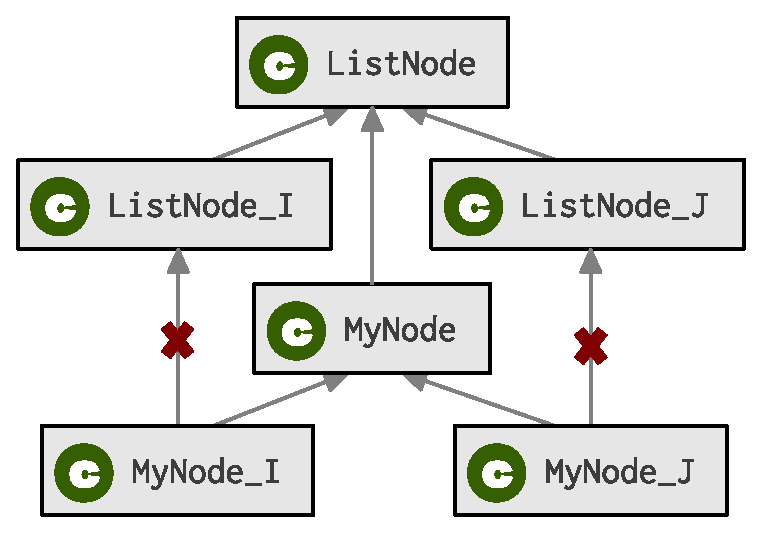
\includegraphics[width=0.30\textwidth]{diags/spec-multi.eps}
    %\vspace{-68mm}
    \caption{An example of specialized class inheritance made impossible by the current translation scheme.}
    \label{fig-spec-multi}
    \vspace{-3mm}
\end{figure}

\subsection{Miniboxing in Scala}

In order to apply the miniboxing encoding to Scala, we decided to use the long integer (|Long|) as the storage type of all other primitive value types. Other sets of storage types could also be implemented to improve specific scenarios, such as running on 32-bit architectures (32-bit |Int| and 64-bit |Long|) or using floating-point numerics extensively\footnote{The floating point to integer bit-preserving transformations, which are implemented as intrinsics, do incur a measurable overhead.} (64-bit |Double| and 64-bit |Long|). Still, for the rest of the description, we will use the long integer as the only storage type, in order to be consistent with the current implementation of the miniboxing plugin.

\topic{The transformation primitives from value types to} |Long| and back are implemented in the HotSpot Java Virtual Machine and have direct translations to bytecode$^\text{4}$ and to processor instructions \cite{intel-ia-32-instruction-reference}. Nevertheless, two concerns need our attention when using miniboxing: %% TODO: Ugly hardcoded footnote
\begin{itemize}
\item Packing and unpacking cost;
\item Memory footprint of the miniboxed encoding.
\end{itemize}

\topic{\textbf{Packing and unpacking cost.} Boxing and unboxing accesses the heap memory. The main goal of miniboxing is to eliminate this overhead,} but, in doing so, conversions to and from long integers must not slow down program execution significantly compared to monomorphic code. Our benchmarks show that indeed the overhead is negligible (\S{}\ref{sec-evaluation}).

\topic{\textbf{Memory footprint.} The miniboxed encoding has a memory footprint between that of monomorphic and generic code.} Considering byte as the type argument, the memory footprint of the miniboxed encoding is 8 times larger than the one for monomorphic code, which would store the byte directly. This factor is reduced by specializing bulk storage (arrays) and considering the paddings introduced by the virtual machine. On the other hand, when compared to boxing on 64 bit processors, the factor is exactly 1, as both a pointer and a long integer have 8 bytes. And this does not take into account the heap space occupied by the boxed values themselves. Therefore, all things considered, miniboxing has a memory footprint larger than the monomorphic and heterogeneous translations, but smaller than homogeneous translations based on boxing.

% The next section will present the miniboxing translation.
\section{Miniboxing Transformation}
\label{mbox:sec-mb-traf}

\topic{The miniboxing transformation, which we developed as a Scala compiler plugin, builds upon specialization}, which has been formalized in \cite{iuli-thesis}. It has the same opportunistic and compatible nature and performs class and method duplication in a similar manner. Still, five elements set it apart:

\begin{itemize}
\item the different inheritance scheme (\S\ref{mbox:sec-mb-traf-inheritance})
\item the type bytes for storing encoded types (\S\ref{mbox:sec-mb-traf-type-bytes}, \S\ref{mbox:sec-mb-traf-classes})
\item the use of a shallow type transformation (\S\ref{mbox:sec-mb-traf-shallow})
\item the use of the final peephole transformation (\S\ref{mbox:sec-mb-traf-peephole})
\item the runtime support for miniboxed values (\S\ref{mbox:sec-mb-traf-runtime} and \S\ref{mbox:sec-runtime})
\end{itemize}

\begin{figure}[t]
    \centering
    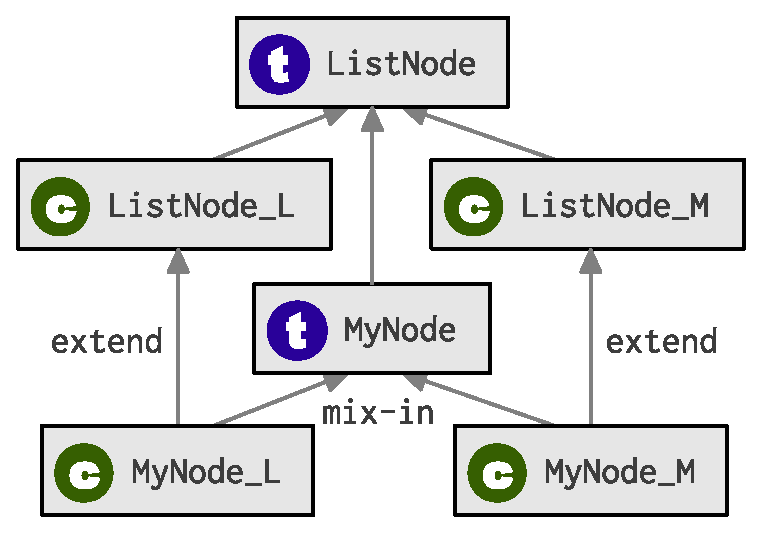
\includegraphics[width=0.50\textwidth]{diags/mbox-multi.eps}

    \caption[Miniboxed inheritance diagram]{An example of miniboxed class inheritance. The suffixes are: M - miniboxed encoding and L - reference type. Compare to the specialized class inheritance in Figure \ref{mbox:fig-spec-multi}.}
    \label{mbox:fig-mbox-multi}
\end{figure}


\subsection{Inheritance}
\label{mbox:sec-mb-traf-inheritance}
\topic{Miniboxing uses a generic trait as the parent of the specialized classes, therefore} avoiding the limitation that miniboxed classes cannot  inherit from each other (\S\ref{mbox:subsec-spec-limits}). Figure \ref{mbox:fig-mbox-multi} shows an example miniboxed class inheritance. As explained in \S\ref{mbox:subsec-spec-limits}, for $n$ specialized type parameters, having a trait as the parent increases the bytecode size from $2^n$ to $4^n$, since each of the $2^n$ miniboxed variants needs to implement all $2^n$ methods. Still, the extra bytecode is well spent, for two reasons:

\begin{itemize}
 \item Having a trait at the top of the hierarchy means no generic fields are inherited in the specialized variants, as it happens when the homogeneous translation is at the top of the hierarchy (\S\ref{mbox:subsec-spec-limits});
 \item This inheritance scheme allows specialized classes to inherit their specialized parent, thus achieving better performance in deep hierarchies.
\end{itemize}

Since the types assigned to tree nodes do not reference the specialized variants but only the generic interface, this inheritance scheme does not interfere with covariance or contravariance. Indeed, if the type parameter of |ListNode| is defined as covariant, |ListNode_M[Int]| is subtype of |ListNode[Int]| and, transitively, of |ListNode[Any]|.

\subsection{Miniboxing Specifics}

This section will work its way from small examples to describing the new elements in the miniboxing transformation, as compared to specialization. In order to simplify the presentation, we will use the |Long|-based encoding for miniboxing, but the transformation can still be generalized to any number of storage types.

\subsubsection*{Type Bytes}
\label{mbox:sec-mb-traf-type-bytes}

In some cases, such as calling the |toString| method on a generic type, the original type of the miniboxed value needs to be recorded. In the current approach, since we only consider primitive types, all we need is an integral type with enough distinct values for each primitive type. In this case, a byte suffices. A more general approach, that also works for value classes, is presented in Section \ref{mbox:subsec-mb-dispatching}, where the encoding descriptor is an object.

The need for type-encoding bytes (or type bytes) is shown by the following example:

\begin{lstlisting-nobreak}
 def print[@minispec T](value: T): Unit = println(value.toString)
\end{lstlisting-nobreak}

Having the type parameter |T| annotated with |@minispec| will trigger miniboxing, which will duplicate this method for |Long|-encoded value types, which we also call miniboxed types. Like specialization, miniboxing produces groups of overloaded methods, with the original method being the all-reference implementation in its group. In our case, only the miniboxed overload needs to be created. To do so, the compiler will create another version of |print| for long integers, which we call |print_M|:

\begin{lstlisting-nobreak}
 def print_M(value: Long): Unit = println(value.toString)
\end{lstlisting-nobreak}

This is a very naive translation. Calling |print(false)|, after method rewiring, will transform the boolean to a long integer whose value will be printed on the screen instead of the ``false'' string. To perform the correct action, the translation should recover the string representation of the boolean value |false| from the |Long| encoding. This suggests the |toString| operation should be rewritten to:

\begin{lstlisting-nobreak}
 def print_M(value: Long): Unit = println(MBRuntime.toString(value))
\end{lstlisting-nobreak}

The code above shows a less naive implementation, since it rewires |toString| calls on the miniboxed value to a special runtime support object in order to obtain the string representation. But passing a single miniboxed value isn't enough, as we mentioned miniboxing does not encode the type with the value as tagged unions do \cite{tagged-unions-lua}. Therefore, it should have a separate parameter to encode the original type:

\begin{lstlisting-nobreak}
 def print_M(T_Type: Byte, value: Long): Unit = println(MBRuntime.toString(value, T_Type))
\end{lstlisting-nobreak}

This is close to the minibox-transformed version of |print_M| the plugin would output. The |T_Type| field only encodes the 9 primitive types in Scala, therefore it does not incur the typical overhead of full reified generics \cite{michel-thesis}. A call to |print(false)| will be translated to the following code, where |BOOLEAN| is the type byte for boolean values:

\begin{lstlisting-nobreak}
 print_M(BOOLEAN, MBRuntime.BoolToMinibox(false))
\end{lstlisting-nobreak}

The method call above shows two differences between rewiring in miniboxing and specialization:
\begin{enumerate}
  \item Calling a miniboxing-transformed method (or instantiating a miniboxing-transformed class) requires passing type bytes for all the |Long|-encoded type arguments;
  \item The arguments to minibox-transformed methods need to be explicitly encoded in the storage type.
\end{enumerate}

We will now present exactly how the miniboxing plugin arrives to this transformed code. As the miniboxing transformation takes place, it needs to preserve program semantics and type correctness. In order to do so, the transformation for |print| is actually done in three steps.

First, the new signature is created, knowing the type parameter |T| is encoded as |Long|. The method name is mangled (mangled names are simplified in this presentation) and the type byte for |T| is added to the signature. Then parameters are added, with all parameters of type |T| being replaced by parameters of type |Long|. As this happens, the symbols whose types changed are recorded and treated specially. In this case, the only miniboxed parameter is |value|, which is recorded. It is also recorded that the type byte |T_Type| corresponds to the encoded type |T|. This yields: (we'll see later why the type parameter |T| still appears)

\begin{lstlisting-nobreak}
 def print_M[T](T_Type: Byte, value: Long): Unit = // need to copy and adapt body from print
\end{lstlisting-nobreak}

In the second step, the body is copied from the |print| method. To maintain type correctness, all the symbols previously recorded as having their types changed are now automatically boxed back to generic type |T|, so the newly generated code tree is consistent in terms of types:

\begin{lstlisting-nobreak}
 def print_M[T](T_Type: Byte, value: Long): Unit = println(MBRuntime.MiniboxToBox[T](value, T_Type).toString)
\end{lstlisting-nobreak}

In the final step, the tree rewrite rules will transform the call to |MiniboxToBox| followed by |toString| into a single call to the |MBRuntime| system, which typically yields better performance:

\begin{lstlisting-nobreak}
 def print_M[T](T_Type: Byte, value: Long): Unit = println(MBRuntime.toString(value, T_Type))
\end{lstlisting-nobreak}

The next section will explain why it is necessary to carry the type parameter |T|.

\subsubsection*{Shallow and Deep Type Transformations}
\label{mbox:sec-mb-traf-shallow}

To further understand the miniboxing transformation, let us look at a more complex example, which builds a linked list with a single element:

\begin{lstlisting-nobreak}
 def list[@minispec T](value: T): ListNode[T] = new ListNode[T](value, null)
\end{lstlisting-nobreak}

As explained before, the |list| method will become the all-reference overload. But the interesting transformation happens in the miniboxed variant. If specialization were to transform this method its signature would be:

\begin{lstlisting-nobreak}
 def list_M[T](value: Long): ListNode[Long]
\end{lstlisting-nobreak}

The return type is incorrect, as we expect |list(3)| to return a |ListNode[Int]|, and yet rewiring |list(3)| to |list_M(...)| would return a |ListNode[Long]|. This exposes the difference between the deep type transformation in specialization and the shallow type transformation in miniboxing: In miniboxing, only values of type |T| are transformed to |Long|, but any type referring to |T|, such as |ListNode[T]|, will remain the same. This explains why the type parameter |T| is carried over to |print_M| and |list_M|: it may still be used in the method's signature and code. The full transformation for method |list_M| will be:

\begin{lstlisting-nobreak}
 def list_M[T](T_Type: Byte, value: Long): ListNode[T] =
   new ListNode[T](MiniboxToBox[T](value, T_Type))
\end{lstlisting-nobreak}

The shallow type transformation also changes types of local variables from |T| to |Long| and recursively transforms all nested methods and classes within the piece of code it is adapting. This propagates the storage type representation throughout the code.

\subsubsection*{Peephole Transformation}
\label{mbox:sec-mb-traf-peephole}

The last transformation to touch the code before it is shipped to the next phase is the peephole transformation, which performs a final sweep over the code to remove redundant conversions. To show this phase at work, let us consider what happens if the |ListNode| class in the last example is also annotated for miniboxing. In this case, the class will have a miniboxed variant, |ListNode_M| to which the instantiation is rewired. Since the |head| parameter of the |ListNode| constructor is boxed, while the |head| parameter of the |ListNode_M| constructor is miniboxed, the transformation will introduce a new |BoxToMinibox| conversion:

\begin{lstlisting-nobreak}
 def list_M[T](T_Type: Byte, value: Long): ListNode[T] =
   new ListNode_M[T](T_Type, BoxToMinibox[T](MiniboxToBox[T](value, ...)), null)
\end{lstlisting-nobreak}

Converting from |Long| to the boxed representation and back before creating the list node will certainly affect performance. Such consecutive complementary conversions and other suboptimal constructs are automatically removed by the peephole optimization: % After the rewrite, the code for |list_M| will be:

\begin{lstlisting-nobreak}
 def list_M[T](T_Type: Byte, value: Long): ListNode[T] =
   new ListNode_M[T](T_Type, value, null)
\end{lstlisting-nobreak}

The code produced by the rewiring phase can be optimized by a single pass of the peephole transformation so there is no need to iterate until a fixed point is reached.

\subsubsection*{Type Bytes in Classes}
\label{mbox:sec-mb-traf-classes}

The class translation is slightly more complex than method translation. For classes, type bytes are also included as fields in the miniboxed variants, to allow the class' methods to encode and decode miniboxed values as necessary: % An example is the translation for the |ListNode| class:

\begin{lstlisting-nobreak}
 class ListNode[@minispec T]
   (val head: T, val tail: ListNode[T]) {
   def contains(element: T): Boolean = ...
 }
\end{lstlisting-nobreak}

The interface resulting after miniboxing will be:

\begin{lstlisting-nobreak}
 trait ListNode[T] {
   ... // getters for head and tail
   def contains(element: T): Boolean
   def contains_M(T_Type_local: Byte, element: Long): Boolean
 }
\end{lstlisting-nobreak}

And the miniboxed variant of this class will be:

\begin{lstlisting-nobreak}
 class ListNode_M[T]
   (T_Type: Byte, head: Long, tail: ListNode[T]) extends ListNode[T] {
   ... // getters for head and tail
   def contains(element: T): Boolean =
         ... // redirect to this.contains_M
   def contains_M(T_Type_local: Byte, element: Long): Boolean =
         ... // specialized implementation
 }
\end{lstlisting-nobreak}

|ListNode_M| has two type tags: |T_Type| is a class parameter and becomes a field of the class while |T_Type_local| is passed to the |contains_M| method directly. In the code example, |T_Type| is used to convert the |element| parameter of |contains| to its miniboxed representation when redirecting the call to |contains_M|. But |T_Type_local| is not used in the |ListNode_M| class. To understand when |T_Type_local| is necessary, we have to look at the re\-fe\-rence-carrying variant of the |ListNode| class:

\begin{lstlisting-nobreak}
 class ListNode_L[T]
   (head: T, tail: ListNode[T]) extends ListNode[T] {
   ... // getters for head and tail
   def contains(element: T): Boolean =
         ... // generic implementation
   def contains_M(T_Type_local: Byte, element: Long): Boolean =
         ... // redirect to this.contains
 }
\end{lstlisting-nobreak}

All instantiations of |ListNode| where the type argument is statically known to be a value type are rewired to |ListNode_M|. The rest of the instantiations are rewired to |ListNode_L|, either because the type argument is not known statically or because it is known to be a reference type. Therefore, there is no reason for |ListNode_L| to carry |T_Type| as a global field. But, in order to allow |contains_M| to decode the miniboxed value |element| into a boxed form and redirect the call |contains|, a local type byte is necessary. Since the |ListNode| interface and its two implementations, |ListNode_L| and |ListNode_M| need to be compatible, the local type byte in |contains_M| is also present for |ListNode_M|, although in the miniboxed class it is redundant.

\subsection{Calling the Runtime Support}
\label{mbox:sec-mb-traf-runtime}

The previous examples have shown how the miniboxing plugin uses the |MBRuntime| object for conversions between unboxed, miniboxed and boxed data representations. But the |MBRuntime| object is not limited to conversions. In Scala, any type parameter is assumed to be a subtype of the |Any| class, so the programmer can invoke methods such as |toString|, |hashCode| and |equals| on generic values. As shown in \S\ref{mbox:sec-mb-traf-type-bytes}, these calls can be translated by a conversion to the boxed representation followed by the call, but are further optimized by calling the implementations in |MBRuntime|, which work directly on miniboxed values.

Aside from conversions and implementations for the methods in the |Any| class, the miniboxing runtime support contains code to allow direct interaction between arrays and miniboxed values. An example that uses arrays is the |ArrayBuffer| class:

\begin{lstlisting-nobreak}
 class ArrayBuffer[@minispec T: Manifest] {
   // fields:
   private[this] var array = new Array[T](32)
   ...
   // methods:
   def getElement(idx: Int): T = array(idx)
   ...
 }
\end{lstlisting-nobreak}

The miniboxed variant |ArrayBuffer_M| is rewritten to call the |MBArray| object to create and access arrays in the miniboxed format:

\begin{lstlisting-nobreak}
 // ArrayBuffer miniboxed variant for primitives:
 class ArrayBuffer_M[T: Manifest](T_Type: Byte)
                               extends ArrayBuffer[T] {
   // fields:
   private[this] var array: Array[T] = MBArray.mbarray_new(32, T_Type)
   ...
   // methods:
   def getElement(idx: Int): T =
       MiniboxToBox(getElement_M(T_Type, idx), ...)
   def getElement_M(T_Type_local: Byte, idx: Int): Long =
       MBArray.array_get(array, idx, T_Type)
   ...
 }
\end{lstlisting-nobreak}

The implementation of the |MBArray| object is critical to numeric algorithms and performance data structures, as it has to be small enough to be inlined by the just-in-time compiler and structured in ways that return the result as fast as possible for any of the primitive types. The following two sections describe the runtime support for arrays and give technical insights into the pitfalls of the implementation.
\section{Miniboxing Bulk Storage Optimization}
\label{mbox:sec-runtime}

Arrays are Java's bulk storage facility. They can store value types or references to heap objects. This is done efficiently, as values are stored one after the other in contiguous blocks of memory and access is done in constant time. Their characteristics make arrays good candidates for internal data structures in collections and algorithms.

But in order to implement compact storage and constant access overhead, arrays are monomorphic under the hood, with separate (and incompatible) variants for each of the primitive value types. What's more, each array type has its own specific bytecode instructions to manipulate it.

The goal we set forth was to match the performance of monomorphic arrays in the context of miniboxing-encoded values. To this end, we had two alternatives to implementing arrays for miniboxed values: use arrays of long integers to store the encoded values or use monomorphic arrays for each type, and encode or decode values at each access.

\topic{Storing encoded values in arrays provides} the advantage of uniformity: all the code in the minibox-specialized class uses the |Long| representation and array access is done in a single instruction. Although this representation wastes heap space, especially for small value types such as boolean or byte, this is not the main drawback: it is incompatible with the rest of the Scala code.

In order to stay compatible with Java, Scala code uses monomorphic arrays for each value type. Therefore arrays of long integers in miniboxed classes must not be allowed to escape from the transformed class, otherwise they may crash outside code attempting to read or write them. To maintain compatibility, we could convert escaping arrays to their monomorphic forms. But the conversion would introduce delays and would break aliasing, as writes from the outside code would not be visible in the miniboxed code and vice versa. Since completely prohibiting escaping arrays severely restricts the programs that can use miniboxing, this solution becomes unusable in practice.

\topic{Thus, the only choice left is to use arrays in their mo\-no\-mor\-phic format for each value type,} so we maintain compatibility with the rest of the Scala code. This decision led to another problem: any array access requires a call to the miniboxing runtime support which performs a dispatch on the type byte. Depending on the type byte's value, the array is cast to its correct type and the corresponding bytecode instruction for accessing it is used. This is followed by the encoding operation, which converts the read value to a long integer. The following snippet shows the array read operation implemented in the miniboxing runtime support code:

\begin{lstlisting-nobreak}
 def array_get[T](array: Array[T], idx: Int, tag: Byte): Minibox = tag match {
   case INT =>
     array.asInstanceOf[Array[Int]](idx).toLong
   case LONG =>
     array.asInstanceOf[Array[Long]](idx)
   case DOUBLE =>  Double.doubleToRawLongBits(
     array.asInstanceOf[Array[Double]](idx)).toLong
   ...
 }
\end{lstlisting-nobreak}

\topic{The most complicated and time-consuming part of our work involved rewriting the miniboxing runtime support to match the performance of specialized code.} The next subsections present the HotSpot Java Virtual Machine execution (\S\ref{mbox:subsec-mb-jvm}), the main benchmark we used for testing (\S\ref{mbox:subsec-mb-bench}) and two implementations for the runtime support: type byte switching (\S\ref{mbox:subsec-mb-switching}) and object-oriented dispatching (\S\ref{mbox:subsec-mb-dispatching}).

\subsection{HotSpot Execution}
\label{mbox:subsec-mb-jvm}

\topic{We used benchmarks to guide our implementation of the miniboxing runtime support.} In this section we will briefly present the just-in-time compilation and optimization me\-cha\-ni\-sms in the HotSpot Java Virtual Machine \cite{hotspot-c1, hotspot-c2}, since they directly influenced our design decisions. Although the work is based on the HotSpot Java Virtual Machine, we highlight the underlying mechanisms that interfere with miniboxing, in hope that our work can be used as the starting point for the a\-na\-ly\-sis on different virtual machines. % , with different heuristics and optimization mechanisms.

\topic{The HotSpot Java Virtual Machine} starts off by interpreting bytecode. After several executions, a method is considered ``hot'' and the just-in-time compiler is called in to transform it into native code. During compilation, aggressive inlining is done recursively on all the methods that have been both executed enough times and are small enough. Typical inlining requirements for the C2\footnote{We did not use tiered compilation.} (server) just-in-time compiler are 10000 executions and size below 35 bytes.

When inlining static calls, the code is inlined directly. For virtual and interface calls, however, the code depends on the receiver. To learn which code to inline, the virtual machine will profile receiver types during the interpretation phase. Then, if a single receiver is seen at runtime, the compiler will inline the method body from that receiver. This inlining may later become incorrect, if a different class is used as the receiver. For such a case the compiler inserts a guard: if the runtime type is not the one expected, it jumps back to interpretation mode. The bytecode may be compiled again later if it runs enough times, with both possible method bodies inlined. But if a third runtime receiver is seen, the call site is marked as megamorphic and inlining is not performed anymore, not even for the previous two method bodies.

After inlining as much code as feasible, the virtual machine's just-in-time compiler applies optimizations, which significantly reduce the running time, especially for array operations which are very regular and for which bounds checks can be eliminated.
\subsection{Benchmark}
\label{mbox:subsec-mb-bench}

We benchmarked the performance on the two examples previously shown before, |ListNode| and |ArrayBuffer|. Throughout benchmarking, one particular method stood out as the most sensitive to the runtime support implementation: the |reverse| method of the |ArrayBuffer| class. The rest of this section uses the |reverse| method to explore the performance of different implementations of the runtime support:

\begin{lstlisting-nobreak}
 def reverse_M(T_Type_local: Byte): Unit = {
   var idx = 0
   val xdi = elemCount - 1
   while (idx < xdi) {
     val el1: Long = getElement_M(T_Type, idx)
     val el2: Long = getElement_M(T_Type, xdi)
     setElement_M(T_Type, idx, el2)
     setElement_M(T_Type, xdi, el1)
     idx += 1
     xdi -= 1
   }
 }
\end{lstlisting-nobreak}

%\newcommand{\optpm}[1]{\optpm{#1}
\newcommand{\optpm}[1]{}

\begin{table}[t!]
\centering
\small
\begin{tabular}{l|r|r}
                                        &   Single Context          & Multi Context          \\\hline
generic                                 &            20.4 \optpm{3.7}&             21.5 \optpm{2.2}\\
miniboxed, no inlining                  &            34.5 \optpm{3.1}&             34.4 \optpm{2.2}\\
\rowcolor{Gray}
miniboxed, full switch                  &             2.4 \optpm{0.6}&             15.1 \optpm{3.5}\\
miniboxed, semi-switch                  &             2.4 \optpm{0.4}&             17.2 \optpm{3.0}\\
miniboxed, decision tree                &            24.2 \optpm{3.0}&             24.1 \optpm{2.9}\\
miniboxed, linear                       &            24.3 \optpm{3.0}&             22.9 \optpm{4.0}\\
\rowcolor{Gray}
miniboxed, dispatcher                   &             2.1 \optpm{0.6}&             26.4 \optpm{1.9}\\
specialized                             &             2.0 \optpm{0.6}&              2.4 \optpm{0.4}\\
monomorphic                             &             2.1 \optpm{0.6}&              N/A  \\
\end{tabular}
\caption{The time in milliseconds necessary for reversing an array buffer of 3 million integers. Performance varies based on how many value types have been used before (Single Context vs. Multi Context).}
\label{mbox:tbl-mb-simple}
\end{table}

The running times presented in table \ref{mbox:tbl-mb-simple} correspond to reversing an integer array buffer of 3 million elements. To put things into perspective, along with different designs, the table also provides running times for monomorphic code (specialized by hand), specialization-annotated code and generic code. Measurements are taken in two scenarios: For ``Single Context'', an array buffer of integers is created and populated and its |reverse| method is benchmarked. In ``Multi Context'', the array buffer is instantiated, populated and reversed for all primitive value types first. Then, a new array buffer of integers is created, populated and its |reverse| method is benchmarked. The HotSpot Java Virtual Machine optimizations are influenced by the historical paths executed in the program, so using other type arguments can have a drastic impact on performance, as can be seen from the table, where the times for ``Single Context'' and ``Multi Context'' are very different: this means the virtual machine gives up some of its optimizations after seeing multiple instantiations with different type arguments.  ``Multi Context'' is the likely scenario a library class will be in, as multiple instantiations with different type arguments may be created during execution.

\subsection{Type Byte Switching}
\label{mbox:subsec-mb-switching}

\topic{The first approach we tried, the simple switch on the type byte, quickly revealed a problem: The array runtime support methods were too large for the just in time compiler to inline at runtime}. This corresponds to the ``miniboxing, no inlining'' in table \ref{mbox:tbl-mb-simple}. To solve this problem, we tasked the Scala compiler with inlining runtime support methods in its backend, independently of the virtual machine. But this was not enough: the |reverse_M| method calls |getElement_M| and |setElement_M|, which also became large after inlining the runtime support, and were not inlined by the virtual machine. This required us to recursively mark methods for inlining between the runtime support and the final benchmarked method.

\topic{The forced inlining in the Scala backend produced good results.} The measurement, corresponding to the ``miniboxed, full switch'' row in the table, shows miniboxed code working at almost the same speed as specialized and monomorphic code. This can be explained by the  loop unswitching optimization in the just-in-time compiler. With all the code inlined by the Scala backend, loop unswitching was able to hoist the type byte switch statement outside the while loop. It then duplicated the loop contents for each case in the switch, allowing array-specific optimizations to bring the running time close to monomorphic code.

\topic{But using more primitive types as type arguments diminished the benefit.} We tested the |reverse| operation in two situations, to check if the optimizations still take place after we use it on array buffers with different type arguments. It is frequently the case that the HotSpot Java Virtual Machine will compile a method with aggressive assumptions about which paths the execution may take. For the branches that are not taken, guards are left in place. Then, if a guard is violated during execution, the native code is interrupted and the program continues in the interpreter. The method may be compiled again later, if it is executed enough times to warrant compilation to native code. Still, upon recompilation, the path that was initially compiled to a stub now becomes a legitimate path and may preclude some optimizations. We traced this problem to the floating point encoding, specifically the bit-exact conversion from floating point numbers to integers, that, once executed, prevents loop unswitching.

\topic{We tried different constructions for the miniboxing runtime support:} splitting the match into two parts and having an if expression that would select one or the other (``semi-switch''), transforming the switch into a decision tree (``decision tree'') and using a linear set of 9 if statements (``linear''), all of which appear in table \ref{mbox:tbl-mb-simple}. These new designs either degraded in the multiple context scenario, or provided a bad baseline performance from the beginning. What's more, the fact that the runtime ``remembered'' the type arguments a class was historically instantiated with made the translation unusable in practice, since this history is not only influenced by code explicitly called before the benchmark, but transitively by all code executed since the virtual machine started. % A different solution was necessary.

\subsection{Dispatching}
\label{mbox:subsec-mb-dispatching}

\topic{The results obtained with type byte switching showed that we were committing to a type too late in the execution:} Forced inlining had to carry our large methods that covered all types inside the benchmarked method, where the optimizer had to hoist the switch outside the loop:

\begin{lstlisting-nobreak}
 while (...) {
   val el1: Long = T_Type match { ... }
   val el2: Long = T_Type match { ... }
   T_Type match { ... }
   T_Type match { ... }
 }
\end{lstlisting-nobreak}

\topic{Ideally, this switch should be done as early as possible, even as soon as class instantiation.} This can be done using an object-oriented approach: instead of passing a byte value during class instantiation and later switching on it, we can pass objects which encode the runtime operations for a single type, much like the where objects in PolyJ \cite{myers-polyj}. We call this object the dispatcher. The dispatcher for each value type encodes a common set of operations such as array get and set. For example, |IntDispatcher| encodes the operations for integers:

\begin{lstlisting-nobreak}
 abstract class Dispatcher {
   def array_get[T](arr: Array[T], idx: Int): Long
   def array_update[T](arr: Array[T], idx: Int, elt: Long): Unit
   ...
 }
 object IntDispatcher extends Dispatcher { ... }
\end{lstlisting-nobreak}

Dispatcher objects are passed to the miniboxed class during instantiation and have final semantics. In the |reverse| benchmark, this would replace the type byte switches by method invocations, which could be inlined. Dispatchers make forced inlining and loop unswitching redundant. With the final |dispatcher| field set at construction time, the |reverse_M| inner loop body can have array access inlined and optimized: (``miniboxed,  dispatcher'' in tables \ref{mbox:tbl-mb-simple} and \ref{mbox:tbl-mb-classloading})

\begin{lstlisting-nobreak}
 // inlined getElement:
 val el1: Long = dispatcher.array_get(...)
 val el2: Long = dispatcher.array_get(...)
 // inlined setElement:
 dispatcher.array_update(...)
 dispatcher.array_update(...)
\end{lstlisting-nobreak}

\topic{Despite their clear advantages, in practice dispatchers can be used with at most two different value types.} This happens because the HotSpot Java Virtual Machine inlines the dispatcher code at the call site and installs guards that check the object's runtime type. The inline cache works for two receivers, but if we try to swap the dispatcher a third time, the callsite becomes megamorphic. In the megamorphic state, the |array_get| and |array_set| code is not inlined, hence the disappointing results for the ``Multi Context'' scenario.

\topic{Interestingly, specialization performs equally well in both ``Single Context'' and ``Multi Context'' scenarios.} The explanation lies in the bytecode duplication: each specialized class contains a different body for the reverse method, and the profiles for each method do not interact. Accordingly, the results for integers are not influenced by the other value types used. This insight motivated the load-time cloning and specialization, which is described in the next section.
\begin{table}[t] \centering \small
\begin{tabular}{l|r|r}
                                        &   Single Context          & Multi Context          \\\hline
generic                                 &            20.4 \optpm{3.7}&             21.5 \optpm{2.2}\\
miniboxed, full switch                  &             2.4 \optpm{0.6}&             15.1 \optpm{3.5}\\
\rowcolor{Gray}
mb. full switch, LS                     &             2.5 \optpm{0.5}&     \textbf{2.4} \optpm{0.5}\\
miniboxed, dispatcher                   &             2.1 \optpm{0.6}&             26.4 \optpm{1.9}\\
\rowcolor{Gray}
mb. dispatcher, LS                      &             2.0 \optpm{0.5}&     \textbf{2.7} \optpm{0.1}\\
specialized                             &             2.0 \optpm{0.6}&              2.4 \optpm{0.4}\\
monomorphic                             &             2.1 \optpm{0.6}&              N/A  \\
\end{tabular}
\caption[Performance results for reversing an array buffer, using class loading]{The time in milliseconds necessary for reversing an array buffer of 3 million integers. Miniboxing benchmarks ran with the double factory mechanism and the load-time specialization are marked with LS. \label{mbox:tbl-mb-runtime}}
\label{mbox:tbl-mb-classloading}
\end{table}

\section{Miniboxing Load-time Optimization}
\label{mbox:sec-classloading}

The miniboxing runtime support, in both incarnations, using switching and dispatching, fails to deliver performance in the ``Multi Context'' scenario. This problem has been addressed in the latest version of the miniboxing plugin by rewriting the accessors in Java as static methods, for which the HotSpot JIT inlining heuristics are more favorable. However, in this section we describe our initial approach, namely to use a load-time transformation, which we abandoned later in the development cycle.

The reason for the poor performance in the ``Multi Context'' scenario, in both incarnations of the runtime support, is that execution takes multiple paths through the code and this prevents the Java Virtual Machine from optimizing. Therefore an obvious solution is to duplicate the class bytecode, but instead of duplicating it on the disk, as specialization does, we do it in memory, on-demand and at load-time. The .NET Common Language Runtime \cite{ecma-dotnet, dot-net-generics} and the OpenJDK Project Valhalla \cite{valhalla-model2-announcement,goetz-specialization} both perform on-demand specialization at load-time, but they do so using more complex transformations encoded in the virtual machine. Instead, we use Java's classloading mechanism.

\topic{We use a custom classloader to clone and specialize miniboxed classes.} Similar to the approach in {\em Pizza} \cite{pizza}, the classloader takes the name of a class that embeds the type byte value. For example, |ListNode_I| corresponds to a clone of |ListNode_M| with the type byte set to |INT|. From the name, the classloader infers the miniboxed class name and loads it from the classpath. It clones its bytecode and adjusts the constant table \cite{jsr-202}. All this is done in-memory.

Once the bytecode is cloned, the paths taken through the inlined runtime support in each class remain fixed during its lifetime, making the performance in ``Single Context'' and ``Multi Context'' comparable, as can be seen in Table \ref{mbox:tbl-mb-classloading}. The explanation is that the JVM sees different classes, with separate type profiles, for each primitive type.

Aside from bytecode cloning, the classloader also performs class specialization:
\begin{itemize}
\item Replaces the type tag fields by static fields (as the class is already dedicated to a type);
\item Uses constant propagation and dead code elimination to reduce each type tag switch down to a single case, which can be inlined by the virtual machine, thus eliminating the need for forced inlining;
\item Performs load-time rewiring, which is described in the next section.
\end{itemize}

\subsection{Miniboxing Load-time Rewiring}
\label{mbox:subsec-runtime-rewiring}

\topic{When rewiring, the miniboxing transformation follows the same rules set forth by specialization (\S\ref{mbox:subsec-spec-rewiring}).} Load-time cloning introduces a new layer of rewiring, which needs to take the cloned classes into account. The factory mechanism we employ to instantiate cloned and specialized classes (\S\ref{mbox:subsec-runtime-instantiation}) is equivalent to the instance rewiring in specialization. The two other rewiring steps in specialization are method rewiring and parent class rewiring. Fortunately method rewiring is done during compilation and since methods are not modified, there is no need to rewire them in the classloader. Parent classes, however, must be rewired at load-time to avoid performance degradation.

Load-time parent rewiring allows classes to inherit and use miniboxed methods while keeping type profiles clean. If the parent rewiring is done only at compile-time, all classes extending |ArrayBuffer_M| share the same code for the |reverse_M| method. But since they may use different type arguments when extending |ArrayBuffer|, they are back to the ``Multi Context'' scenario in table \ref{mbox:tbl-mb-simple}. To obtain good performance, rewiring parent classes is done first at compile time, to the miniboxed variant of the class, and then at load-time, to the cloned and specialized class.

A good question at this point is, given a load-time transformation, why should we still perform the miniboxing transformation during compilation? The answer is that, once the class has been miniboxed, the transformation is as simple as hard-coding the type byte into the loaded class and running simple constant propagation and dead code elimination optimization phases on the bytecode to eliminate redundant branches. Instead, if we were to keep the generic information at the bytecode level, the bytecode format would have to be updated and the load-time transformations would be more complex.

The following snippet shows parent rewiring in the case of dispatcher objects:

\begin{lstlisting-nobreak}
 // user code:
 class IntBuff extends ArrayBuffer[Int]
 // after compile-time rewiring:
 class IntBuff extends ArrayBuffer_M[Int](IntDispatcher)
 // after load-time rewiring:
 class IntBuff extends ArrayBuffer_I[Int](IntDispatcher)
\end{lstlisting-nobreak}

\topic{The load-time rewiring of parent classes requires all subclasses with miniboxed parents to go through the classloader transformation.} This includes the classes extending miniboxed parents with static type arguments, such as the |IntBuff| class in the code snippet before. This incurs a first-instantiation overhead, which is an inconvenience especially for classes that are only used once, such as anonymous closures extending |FunctionX|. But not all classes make use of the miniboxing runtime for arrays, so we can devise an annotation which hints to the compiler which classes need factory instantiation. This would only incur the cloning and specialization overhead when the classes use arrays. The annotation could be automatically added by the compiler when a class uses array operations and propagated from parent classes to their children:

\begin{lstlisting-nobreak}
 @loadtimeSpec
 class ArrayBuffer[@minispec T]

 // IntBuff automatically inherits @loadtimeSpec
 class IntBuff extends ArrayBuffer[Int]
\end{lstlisting-nobreak}

\subsection{Efficient Instantiation}
\label{mbox:subsec-runtime-instantiation}

Imposing the use of a global classloader is impossible in many practical applications. To allow miniboxing to work in such cases, we chose to perform the class instantiation through a factory that loads a local specializing classloader, requests the cloning and specialization of the miniboxed class and instantiates it via reflection. We benchmarked the approach and it introduced significant overhead, as instantiations using reflection are very expensive.

\topic{To counter the cost of reflective instantiation,} we propose a ``double factory'' approach that uses a single reflective instantiation per cloned class. In this approach each cloned and specialized class has a corresponding factory -- that instantiates it using the {\bf new} keyword. When instantiating a miniboxed class with a new set of type arguments, its corresponding factory is specialized by the classloader and instantiated via reflection. From that point on, any new instance is created by the factory, without the reflective delay. The following code snippet shows the specialized (or 2$^\text{nd}$ level) factory:

\begin{lstlisting-nobreak}
 // Factory interface
 abstract class ArrayBufferFactoryInterface {
   def newArrayBuffer_M[T: Manifest](disp: Dispatcher[T]): ArrayBuffer[T]
 }
 // Factory instance, to be specialized
 // in the classloader
 class ArrayBufferFactoryInstance_M extends ArrayBufferFactoryInterface {
   def newArrayBuffer_M[T: Manifest](disp: Dispatcher[T]): ArrayBuffer[T] =
     new ArrayBuffer_M(disp)
 }
\end{lstlisting-nobreak}

\section{Evaluation}
\label{mbox:sec-evaluation}

%%%%%%%%%%%% STUFF FOR TABLE %%%%%%%%%%%%
\newcolumntype{C}{>{\centering\arraybackslash}p{14ex}}
%\newcolumntype{X}{>{\centering\arraybackslash}p{5ex}}
%\newcommand{\optpm}[1]{$\pm$ #1}
%\newcommand{\optpm}[1]{}
\newcommand{\sctx}[0]{Single Ctx.}
\newcommand{\mctx}[0]{Multi Ctx.}
\newcommand{\bn}[1]{\textbf{#1}}
\newcommand{\opt}[1]{#1}
%\newcommand{\opt}[1]{}

This section presents the results obtained by the miniboxing transformation. It will first present the miniboxing compiler plug-in and the miniboxing classloader (\S\ref{mbox:subsec-eval-impl}). Next, it will present the benchmarking infrastructure (\S\ref{mbox:subsec-eval-infrastructure}) and the benchmark targets (\S\ref{mbox:subsec-eval-targets}). Finally, it will present the results (\S\ref{mbox:subsec-eval-results} - \S\ref{mbox:subsec-eval-other-vms}) and draw conclusions (\S\ref{mbox:subsec-eval-remarks}).

\subsection{Implementation}
\label{mbox:subsec-eval-impl}

\topic{The miniboxing plug-in adds a code transformation phase in the Scala compiler.} Like specialization, the miniboxing phase is composed of two steps: transforming signatures and transforming trees. As the signatures are specialized, metadata is stored on exactly how the trees need to be transformed. This metadata later guides the tree transformation in duplicating and adapting the trees to obtain the miniboxed code. The duplication step reuses the infrastructure from specialization, with a second adaptation step which transforms storage from generic to miniboxed representation.

The plugin performs several transformations:
\begin{itemize}
\item Code duplication and adaptation, where values of type |T| are replaced by long integers and are un-miniboxed back to |T| at use sites (\S\ref{mbox:sec-mb-traf-type-bytes});
\item Rewiring methods like |toString|, |hashCode|, |equals| and array operations to use the runtime support (\S\ref{mbox:sec-mb-traf-runtime});
\item Opportunistic rewiring: new instance creation, specialized parent classes and method invocations (\S\ref{mbox:subsec-spec-rewiring});
\item Peephole minibox/un-minibox reduction (\S\ref{mbox:sec-mb-traf-peephole}).
\end{itemize}

\topic{The miniboxing classloader} duplicates classes and performs the specialized class rewiring. It uses transformations from an experimental Scala backend to perform constant propagation and dead code elimination in order to remove switches on the type byte. It supports miniboxed classes generated by the current plug-in and in the current release only works for a single specialized type parameter. Also, the infrastructure for the double factory instantiation was written and tuned by hand, and may be integrated in the plug-in in a future release. We did not implement the |@loadtimeSpec| annotation yet.

\topic{The project also contains code for testing the plug-in and the classloader and performing microbenchmarks,} something which turned out to be more difficult than expected.

\subsection{Benchmarking Infrastructure}
\label{mbox:subsec-eval-infrastructure}

\topic{The miniboxing plug-in produces bytecode which is then executed by the HotSpot Java Virtual Machine.} Although the virtual machine provides useful services to the running program, such as compilation, deoptimization and garbage collection, these operations influence our microbenchmarks by delaying or even changing the benchmarked code altogether. Furthermore, the non-deterministic nature of such events make proper benchmarking harder \cite{rigorous-java-benchmarking}.

\topic{In order to have reliable results for our microbenchmarks, we used ScalaMeter \cite{scalameter},} a tool specifically designed to reduce benchmarking noise. ScalaMeter is currently used in performance-testing the Scala standard library. When benchmarking, it forks a new virtual machine such that fresh code caches and type profiles are created. It then warms up the benchmarked code until the virtual machine compiles it down to native code using the C2 (server) \cite{hotspot-c2} compiler. When the code has been compiled and the benchmark reaches a steady state, ScalaMeter measures several execution runs. The process is repeated several times, 100 in our case, reducing the benchmark noise. For the report, we present the average of the measurements performed.

\topic{We ran the benchmarks} on an 8-core i7 machine running at 3.40GHz with 16GB of RAM memory. The machine ran a 64 bit version of Linux Ubuntu 12.04.2. For the Java Virtual Machine we used the Oracle Java SE Runtime Environment build 1.7.0\_11 using the C2 (server) compiler. The following section will describe the benchmarks we ran.

\subsection{Benchmark Targets}
\label{mbox:subsec-eval-targets}

We executed the benchmarks in two scenarios:
\begin{itemize}
\item ``Single Context'' corresponds to the benchmark target (|ArrayBuffer| or |ListNode|) executed with a single value type, |Int|;
\item ``Multi Context'' corresponds to running the benchmark for all value types and only then measuring the execution time for the target value type, |Int|;
\end{itemize}

The benchmarks were executed with 7 transformations:
\begin{itemize}
\item {generic}: the generic version of the code, uses boxing;
\opt{\item {mb. switch}: miniboxed, using the type byte switching};
\opt{\item {mb. dispatcher}: miniboxed, dispatcher runtime support};
\item {mb. switch + LS}: miniboxed, type byte switching, load-time specialization with the double factory mechanism;
\item {mb. dispatcher + LS}: miniboxed, dispatcher, load-time specialization with the double factory mechanism;
\item {specialized}: code transformed by specialization;
\item {monomorphic}: code specialized by hand, which does not need the redirects generated by specialization.
\end{itemize}


\topic{For the benchmarks, we used the two classes presented in the previous sections:} The |ArrayBuffer| class simulates collections and algorithms which make heavy use of bulk storage and the |ListNode| class simulates collections which require random heap access. We chose the benchmark methods such that each tested a certain feature of the miniboxing transformation. We used very small methods such that any slowdowns can easily be attributed to bytecode or can be diagnosed in a debug build of the virtual machine, using the compilation and deoptimization outputs.

|ArrayBuffer.append| creates a new array buffer and appends 3 million elements to it. This benchmark tests the array writing operations in isolation, such that they cannot be grouped together and optimized.

|ArrayBuffer.reverse| reverses a 3 million element array buffer. This benchmark proved the most difficult in terms of matching the monomorphic code performance.

|ArrayBuffer.contains| checks for the existence of elements inside an initialized array buffer. It exercises the |equals| method rewiring and revealed to us that the initial transformation for |equals| was suboptimal, as we were not using the information that two miniboxed values were of the same type. This benchmark showed a 22x speedup over generic code.

List construction builds a 3 million element linked list using |ListNode| instances. This benchmark verifies the speed of miniboxed class instantiation. It was heavily slowed down by the reflective instantiation, therefore we introduced the double factory for class instantiation using the classloader.

|List.hashCode| computes the hash code of a list of 3 million elements. We used this benchmark to check the performance of the |hashCode| rewiring. It was a surprise to see the |hashCode| performance for generic code running in the interpreter (Table \ref{mbox:tbl-results-interp}). It is almost one order of magnitude faster than specialized code and 5 times faster than miniboxing. The explanation is that computing the hash code requires boxing and calling the |hashCode| method on the boxed object. When the benchmarks are compiled and optimized, this is avoided by inlining and escape analysis, but in the interpreter, the actual object allocation and call to |hashCode| do happen, making the heterogeneous translation slower.

|List.contains| tests whether a list contains an element, repeated for 3 million elements. It tests random heap access and the performance of the |equals| operator rewiring.

\subsection{Benchmark Results}
\label{mbox:subsec-eval-results}

\begin{table}[t!]
\centering
\footnotesize
\begin{tabularx}{\textwidth}{l| *{6}{|Y}}
                  & \multicolumn{2}{c|}{\scriptsize \texttt{ArrayBuffer.append}} & \multicolumn{2}{c|}{\scriptsize \texttt{ArrayBuffer.reverse}} & \multicolumn{2}{c}{\scriptsize\texttt{ArrayBuffer.contains}} \\\hline
                  & \sctx            & \mctx            & \sctx            & \mctx            & \sctx                & \mctx            \\\hline
generic           & 50.1 \optpm{1.2} & 48.0 \optpm{0.9} & 20.4 \optpm{3.8} & 21.5 \optpm{2.3} & 1580.1 \optpm{ 12.0} &  3628.8 \optpm{ 40.2} \\
\opt{mb. switch        & 30.9 \optpm{2.0} & 35.5 \optpm{2.4} &  2.5 \optpm{0.5} & 15.1 \optpm{3.5} &  161.5 \optpm{  3.4} &   554.3 \optpm{  3.2} \\}
\opt{mb. dispatch      & 16.5 \optpm{1.3} & 58.2 \optpm{3.0} &  2.1 \optpm{0.6} & 26.5 \optpm{1.9} &  160.7 \optpm{  3.0} &  2551.6 \optpm{ 33.1} \\}
\rowcolor{Gray}
\bn{mb. switch + LS}   & \bn{15.6} \optpm{1.8} & \bn{14.8} \optpm{1.5} &  \bn{2.5} \optpm{0.5} &  \bn{2.4} \optpm{0.5} &  \bn{159.9} \optpm{  3.2} &   \bn{161.7} \optpm{  3.4} \\
\rowcolor{Gray}
\bn{mb. dispatch + LS} & \bn{15.1} \optpm{0.9} & \bn{15.9} \optpm{1.5} &  \bn{2.0} \optpm{0.6} &  \bn{2.7} \optpm{0.1} &  \bn{161.8} \optpm{  2.2} &   \bn{161.3} \optpm{  2.8} \\
specialization    & 39.7 \optpm{3.0} & 38.5 \optpm{3.0} &  2.0 \optpm{0.6} &  2.4 \optpm{0.5} &  155.8 \optpm{  2.6} &   156.3 \optpm{  3.4} \\
monomorphic       & 16.2 \optpm{1.0} & N/A           &  2.1 \optpm{0.6} & N/A           &  157.7 \optpm{  4.1} &                N/A \\[0.1em]

                  & \multicolumn{2}{c|}{{\scriptsize \texttt{List}} creation} & \multicolumn{2}{c|}{\scriptsize \texttt{List.hashCode}} & \multicolumn{2}{c}{\scriptsize \texttt{List.contains}} \\\hline
                  & \sctx            & \mctx            & \sctx            & \mctx            & \sctx                & \mctx            \\\hline
generic           & 16.7 \optpm{   0.2} & 1841 \optpm{ 1068} & 22.1 \optpm{1.9} & 20.4 \optpm{0.8} & 1739.5 \optpm{ 4.9} & 2472.4 \optpm{49.0} \\
\opt{mb. switch        & 11.4 \optpm{   0.1} &  11.7 \optpm{   0.6} & 18.3 \optpm{2.2} & 18.8 \optpm{2.2} & 1438.2 \optpm{17.5} & 1443.2 \optpm{21.8} \\}
\opt{mb. dispatch      & 11.4 \optpm{   0.1} &  11.5 \optpm{   0.4} & 15.6 \optpm{1.8} & 21.0 \optpm{1.9} & 1369.1 \optpm{ 8.0} & 1753.2 \optpm{16.9} \\}
\rowcolor{Gray}
\bn{mb. switch + LS}   & \bn{11.5} \optpm{   0.6} &  \bn{11.6} \optpm{   0.5} & \bn{16.2} \optpm{2.4} & \bn{16.1} \optpm{2.2} & \bn{1434.9} \optpm{20.4} & \bn{1446.3} \optpm{19.6} \\
\rowcolor{Gray}
\bn{mb. dispatch + LS} & \bn{12.1} \optpm{   0.5} &  \bn{12.7} \optpm{   1.9} & \bn{16.1} \optpm{2.1} & \bn{15.3} \optpm{1.7} & \bn{1364.2} \optpm{ 7.8} & \bn{1325.9} \optpm{44.4} \\
specialization    & 11.4 \optpm{   0.1} &  11.4 \optpm{   0.2} & 14.5 \optpm{1.4} & 36.4 \optpm{2.5} & 1341.0 \optpm{37.8} & 1359.2 \optpm{23.4} \\
monomorphic       & 10.2 \optpm{   1.2} &                 N/A  & 13.3 \optpm{0.8} & N/A              & 1172.0 \optpm{ 3.4} & N/A                 \\
\end{tabularx}
\caption[Miniboxing benchmark running times on HotSpot with C2 compiler]{Benchmark running times. The benchmarking setup is presented in \S\ref{mbox:subsec-eval-infrastructure} and the targets are presented in \S\ref{mbox:subsec-eval-targets}. The time is measured in milliseconds.}
\label{mbox:tbl-results-main}
\end{table}

Table \ref{mbox:tbl-results-main} presents the main results of our benchmarks. The table highlights  ``mb. switch + LS'' and ``mb. dispatch + LS'', which represent the miniboxing encoding using the load-time specialization invoked with the double factory mechanism.

The miniboxing encoding based on type tag switching, ``mb. switch + LS'', offers steady performance close to that of specialization and monomorphic code, with slowdowns ranging between 0 and 20 percent. The classloader specialization, coupled with constant propagation and dead code elimination, make the type tag switching approach the most stable across multiple executions with different type arguments, with at most 6 percent difference between ``Single Context'' and ``Multi Context'', in the case of |ArrayBuffer.append|.

The dispatcher-based encoding, ``mb. dispatch + LS'', also offers performance close to specialization and mono\-morphic code, with slightly better performance when traversing the linked list (benchmarks |hashCode| and |contains|), and a lower performance on |List| creation. This suggests that passing the dispatcher object on the stack is more expensive than passing a type tag.

It is worth noting that the dispatcher-based implementation relies on inlining performed by the just-in-time compiler. Although the load-time cloning mechanism ensures type profiles remain monomorphic, the burden of inlining falls on the just-in-time compiler. In the case of virtual machines that perform ahead-of-time compilation, such as Excelsior JET \cite{excelsior-jet}, the newly specialized class is compiled to native code without interpretation, thus no type profiles are available and no inlining takes place for the miniboxing runtime. In contrast to dispatching, type tag switching only requires loading-time constant propagation and dead code elimination to remove the overhead of the miniboxing runtime. This makes it a better candidate for robust performance across different virtual machines. The next section will present interpreter benchmarks.

\subsection{Interpreter Benchmarks}
\label{mbox:subsec-eval-interpreter}

\begin{table}[t!]
\centering
\small
\begin{tabular}{l|c|c|c|c|c|c}
                  & \multicolumn{3}{c|}{\texttt{ArrayBuffer}} & \multicolumn{3}{c}{\texttt{List}} \\\hline
generic           & 4.6 & 2.2 & 367.0 & 1.4 & \textbf{0.2} & 16.6 \\
\rowcolor{Gray}
\bn{mb. switch + LS}   & \bn{1.6} & \bn{0.3} &  \bn{25.0} & \bn{0.8} & \bn{1.3} &  \bn{4.2} \\
mb. dispatch + LS & 2.5 & 0.7 &  88.9 & 1.1 & 1.5 &  7.3 \\
specialization    & 4.3 & 0.5 &  30.7 & 0.6 & 1.9 &  2.2 \\
monomorphic       & 1.0 & 0.2 &  12.7 & 0.4 & 1.2 &  2.2 \\
\end{tabular}
\caption[Miniboxing benchmark running times on HotSpot interpreter]{Running time for the benchmarks in the HotSpot Java Virtual Machine interpreter. The time is measured in seconds as instead of milliseconds as in the other tables. ``Single context'' and ``Multi context'' have similar results.}
\label{mbox:tbl-results-interp}
\end{table}

Before compiling the bytecode to native machine code, the HotSpot Virtual Machine interprets it and gathers profiles that later guide compilation. Table \ref{mbox:tbl-results-interp} presents results for running the same set of benchmarks in the interpreter, without compilation. It is important that transformations do not visibly degrade performance in the interpreter, as this slows down application startup. The data highlights a steady behavior for the the type tag switching, while the dispatcher-based approach suffers from up to 4x slowdowns.

The data shows a consistent slowdown of the tag switching approach compared to the monomorphic code in 4 of the 6 experiments. This can most likely be attributed to the mechanism for invoking object methods, which requires loading a reference to the module from a static field and then performing a method call. Even after the method call is inlined, the Scala backend (and the load-time specializer) do not remove the static field access, thus leaving the redundant but possibly side-effecting instruction in the hot loop. In the native code the field access is compiled away by the just-in-time compiler. This could be improved in the Scala backend.

\begin{table}[b!]
\centering
\small
\begin{tabular}{l|r|r|g|r}
                      &   erasure  &   dispatch &    switch &        spec. \\\hline
ArrayBuffer           &        4.4 &       19.5 &      24.5 &         57.6 \\
ArrayBuffer factory   &         -- &      + 9.0 &     + 8.5 &           -- \\
ListNode              &        3.1 &       10.9 &      11.5 &         45.0 \\
ListNode factory      &         -- &      + 8.7 &     + 8.3 &           -- \\
\end{tabular}
\caption[Bytecode generated for different translations]{Bytecode generated by different translations, in kilobytes. Factories add extra bytecode for the double factory mechanism. ``spec.'' stands for specialization.}
\label{mbox:tbl-results-bytecode}
\end{table}

\begin{table}[t!]
\centering
\small
\begin{tabular}{l|r|r}
                               &  bytecode size (KB) & classes \\\hline
Spire - specialized (current)  &               13476 &    2545 \\
\rowcolor{Gray}
Spire - miniboxed              &                4820 &    1807 \\
Spire - generic                &                3936 &    1530 \\
\end{tabular}
\caption[Bytecode size comparison: generic, miniboxing and specialization (Spire)]{Bytecode generated by using specialization, miniboxing and leaving generic code in the Spire numeric abstractions library.}
\label{mbox:tbl-results-bytecode-spire}
\end{table}

\begin{table}[b!]
\centering
\small
\begin{tabular}{l|r|r}
                               &  bytecode size (KB) & classes \\\hline
Vector - specialized           &                5691 &    1434 \\
\rowcolor{Gray}
Vector - miniboxed             &                1210 &     435 \\
Vector - generic (current)     &                 715 &     223 \\
\end{tabular}
\caption[Bytecode size comparison: generic, miniboxing and specialization (Vector)]{Bytecode generated by using specialization, miniboxing and leaving generic code on the Scala collection library slice around Vector.}
\label{mbox:tbl-results-bytecode-vector}
\end{table}

\subsection{Bytecode Size}
\label{mbox:subsec-eval-size}

Table \ref{mbox:tbl-results-bytecode} presents the bytecode generated for |ArrayBuffer| and |ListNode| by 4 transformations: erasure, miniboxing with dispatcher, miniboxing with switching and specialization. The fraction of bytecode created by miniboxing, when compared to specialization, lies between 0.2x to 0.4x. This is marginally better than the fraction we expected, 0.4x, which corresponds to $4^n / 10^n$ for $n=1$. The reason the fraction is $4^n / 10^n$ instead of $2^n / 10^n$ is explained in \S \ref{mbox:sec-mb-traf-inheritance}. The double factory mechanism adds a significant bytecode, in the order of 10 kilobytes per class.

In order to evaluate the benefits of using the miniboxing encoding for real-world software, we developed a ``specialization-hijacking'' mode, where specialization was turned off and all |@specialized| notations were treated as |@minispec|, thus triggering miniboxing on all methods and classes where specialization was used. For this benchmark we only used the switching-based transformation.

The first evaluation was performed on Spire \cite{erik-spire}, a Scala library providing abstractions for numeric types, ranging from boolean algebras to complex number algorithms. Spire is the one library in the Scala community which uses specialization the most, and the project owner, Erik Osheim, contributed numerous bug fixes and enhancements to the Scala compiler in the area of specialization. The results, presented in Table \ref{mbox:tbl-results-bytecode-spire}, show a bytecode reduction of 2.8x and a 1.4x, or 40\%, reduction in the number of specialized classes. The two reductions are not proportional because specialized methods inflate the code size of classes, but do not increase the class count. The bytecode reduction is limited to 2.8x because specialization is used in a directed manner, pointing exactly to the value types which should be specialized. So, instead of generating 10 classes per type parameter, it only generates the necessary value types. Nevertheless, even starting from manually directed specialization, the miniboxing transformation is able to further reduce the bytecode size.

The second evaluation, shown in Table \ref{mbox:tbl-results-bytecode-vector}, is motivated by a common complaint in the Scala community: that the collections in the standard library should be specialized. To perform an evaluation on collections, we sliced a part of the library around the |Vector| class and examined the impact of using the specialization and miniboxing transformations. On the approximately 64 Scala classes, traits and objects included in our slice, the bytecode reduction obtained by miniboxing compared to specialization is 4.7x. Compared to the generic |Vector|, the miniboxing code growth is 1.7x, opposed to almost 8x for specialization.


\subsection{Load-time Specialization Overhead}
\label{mbox:subsec-eval-specialization}

In this section we will evaluate the overhead of the double factory mechanism. There are three types of overhead involved:
\begin{itemize}
  \item Bytecode overhead, shown in the previous section;
  \item Time spent specializing and loading a class;
  \item Heap overhead for the classloader and factory.
\end{itemize}

We will further explore the last two sources of overhead.

\begin{table}[t!]
\centering
\small
\begin{tabular}{l @{\hspace{11mm}} |r|r}
                                    & time in ms   & classes \\\hline
classpath - just load               &  182 $\pm$ 5 &     9 $\times$ 25 = 225 \\
classloader - warmed up             &  300 $\pm$ 4 &     225 \\
classloader - cold start            &  461 $\pm$ 9 &     225 \\
\end{tabular}
\caption[Class loading time: loading, cloning and specialization]{Loading time (classpath) and time for cloning and specialization (classloader) for the 9 specialized variants of Vector and their transitive dependencies.}
\label{mbox:tbl-results-classloading-load}
\end{table}

\begin{table}[b!]
\centering
\small
\begin{tabular}{l @{\hspace{7mm}} |r|r}
                               & time in ms   & classes \\\hline
classpath - new                &  258 $\pm$ 5 &     9 $\times$ 42 = 378 \\
classpath - factory            &  268 $\pm$ 6 &     378 \\
classloader - factory - warm   &  488 $\pm$10 &     378 \\
classloader - factory - cold   &  655 $\pm$ 9 &     378 \\
\end{tabular}
\caption[Instantiation time: loading, cloning, specialization and instantiation]{Instantiation time for the 9 specialized variants of Vector and their transitive dependencies.}
\label{mbox:tbl-results-classloading-inst}
\end{table}

\subsubsection*{Time Spent Specializing}

Table \ref{mbox:tbl-results-main}, in the ``|List| creation'' column, shows the overhead of the double factory mechanism and class specialization is not statistically noticeable after the mechanism is warmed up. Nevertheless, it is important to understand how the mechanism behaves during a cold start, as this directly impacts an application's startup time. In this subsection we will examine the overhead for a cold start, coming from two different sources:

\begin{itemize}
  \item The runtime class specialization;
  \item The cold start of the double factory mechanism.
\end{itemize}

The evaluation checks the two overheads separately: in the first experiment we only load the classes (using |Class.forName|) to trigger the runtime class specialization, while in the second experiment we instantiate the classes, either directly, using the |new| operator or through the double factory mechanism. In order to evaluate the class specialization, we instrumented the specializing classloader to dump the resulting class files, such that we can compare the specializing classloader to simply loading the specialized variants from the classpath.

For the comparison, we use the |Vector| class described in the previous section. The |Vector| class mixes in 36 traits \cite{scalable-component-abstractions} which are translated by the Scala compiler as transitive dependencies of the class. In our experiments, loading the |Vector| class using |Class.forName| transitively loaded another 24 specialized classes for each variant. Instantiating a vector using |new| further loads another 18 classes, mainly specialized trait implementations and internal classes, leading to a total of 42 classes loaded with each specialized variant of |Vector|.

In each experiment we start the virtual machine, start counting the time, load or instantiate |Vector| for all 9 value types in Scala, output the elapsed time and exit. Once a class is loaded, its internal representation in the virtual machine remains cached until its classloader is garbage collected. In order to perform correct benchmarks, we chose to use a virtual machine to load the 9 specialized variants of |Vector| only once, and then restart the virtual machine. We repeated the process 100 times for each measurement.

The first experiment involves loading the class: this can be done either by using the specializing classloader to instantiate a template or by loading the class file dumped from a previous specialization run. We observed a significant difference between cold starting the specializing classloader and warming it up on a different set of classes. This is shown in Table \ref{mbox:tbl-results-classloading-load}: cold starting the specialization classloader incurs a slowdown of 153\% while warming it up before leads to a 65\% slowdown in class loading time.

The second experiment involves instantiating the class, either directly (using the |new| operator) or through the double factory mechanism. Table \ref{mbox:tbl-results-classloading-inst} presents the results. The surprising result of this experiment is that the overhead caused by the double factory mechanism is under 4\%. As before, most of the time is spent specializing the template to produce the specialized class, which, depending on whether the classloader was used before, can lead to a slowdown between 84\% and 144\%. It is important to point out this overhead is a one-time cost, and further instantiations of the specialized variants take on the order of tens of milliseconds.

\subsubsection*{Heap Overhead}

In this section we will attempt to bound the heap usage of the double factory mechanism. The double factory mechanism consists of a first level factory, which uses reflection to create second level factories, which, in turn, use the new operator to instantiate load-time specialized classes. This mechanism was imposed in order to avoid the cost of reflection-based instantiation, which we found to be more expensive in terms of overhead. Each second level factory corresponds to a set of pre-determined type tags, thus instantiating two specialized variants will require two separate second level factories.

The first level factory mechanism keeps a cache of $10^n$ references pointing to second level factories, which is initially empty and fills up as the different variants are created. The second level factories are completely stateless and only offer a method for each specialized class constructor. Therefore the maximum heap consumption, for a 64 bit system running the HotSpot Virtual Machine, would be 16 bytes for each second level factory and 8 bytes for its cached reference, all times $10^n$, assuming all variants are loaded. This means a total of $24 \times 10^n$ bytes of storage. For a class with a single type parameter, this would mean a heap overhead in the order of hundreds of bytes. Assuming all of spire's specialized classes used arrays and required the two factory mechanism, since most take a single type parameter, it would mean a heap overhead in the order of tens of kilobytes.

However a hidden overhead is also present, consisting of the internal class representations for the second level factories inside the virtual machine. To bound this overhead, we can compare the factories to the classes themselves: for each specialized variant of the class there will be a specialized factory, with a method corresponding to each constructor of the class. The factory will therefore always have a strictly smaller internal representation than the specialized class, leading to at most a doubling of the internal class representation in the virtual machine.

\begin{table*}[t!]
\centering
\footnotesize

\begin{tabularx}{\textwidth}{l| *{6}{|Y}}
                  & \multicolumn{2}{c|}{\scriptsize \texttt{ArrayBuffer.append}} & \multicolumn{2}{c|}{\scriptsize \texttt{ArrayBuffer.reverse}} & \multicolumn{2}{c}{\scriptsize\texttt{ArrayBuffer.contains}} \\\hline
                       & \sctx            & \mctx            & \sctx            & \mctx            & \sctx                & \mctx            \\\hline
generic                & 78.3 \optpm{12.6}& 52.3 \optpm{2.2} &  3.2 \optpm{1.0} & 20.3 \optpm{1.8} &  607.6 \optpm{  0.6} &  3146.1 \optpm{  4.8} \\
\opt{mb. switch        & 27.6 \optpm{13.8}&         $\times$ &  7.4 \optpm{1.5} &         $\times$ &  844.4 \optpm{  1.0} &              $\times$ \\}
\opt{mb. dispatch      & 27.0 \optpm{2.0} & 34.8 \optpm{1.6} &  3.2 \optpm{0.1} & 10.8 \optpm{1.5} &  844.7 \optpm{  0.6} &   962.7 \optpm{ 1.3} \\}
\rowcolor{Gray}
\bn{mb. switch + LS}   & \bn{22.2} \optpm{9.3} & \bn{14.3} \optpm{1.3} &  \bn{3.8} \optpm{0.8} &  \bn{2.9} \optpm{0.1} &  \bn{725.4} \optpm{  0.7} &   \bn{725.2} \optpm{  0.5} \\
\rowcolor{Gray}
\bn{mb. dispatch + LS} & \bn{32.9} \optpm{8.2} & \bn{26.4} \optpm{2.1} &  \bn{3.4} \optpm{0.3} &  \bn{4.0} \optpm{0.9} &  \bn{844.6} \optpm{  0.9} &   \bn{845.3} \optpm{  3.0} \\
specialization         & 21.7 \optpm{8.3} & 13.4 \optpm{2.1} &  3.5 \optpm{0.7} &  2.7 \optpm{0.8} &  488.7 \optpm{  0.9} &   489.4 \optpm{  2.5} \\
monomorphic            & 19.8 \optpm{5.9} & N/A           &  3.1 \optpm{0.5} & N/A           &  490.4 \optpm{  3.0} &                N/A \\[0.1em]

                  & \multicolumn{2}{c|}{{\scriptsize \texttt{List}} creation} & \multicolumn{2}{c|}{\scriptsize \texttt{List.hashCode}} & \multicolumn{2}{c}{\scriptsize \texttt{List.contains}} \\\hline
                       & \sctx            & \mctx            & \sctx            & \mctx            & \sctx                & \mctx            \\\hline
generic                & 32.6 \optpm{   7.5} &  23.3 \optpm{ 1.5} & 13.4 \optpm{1.7} & 13.6 \optpm{1.2} & 1846.5 \optpm{ 4.9} & 2168.1 \optpm{4.0} \\
\opt{mb. switch        & 23.7 \optpm{   1.2} &  18.0 \optpm{ 0.4} & 11.7 \optpm{1.0} & 10.9 \optpm{0.4} & 1420.8 \optpm{15.3} & 1421.5 \optpm{16.0} \\}
\opt{mb. dispatch      & 20.9 \optpm{   1.9} &  18.3 \optpm{ 1.0} & 12.4 \optpm{0.9} & 11.4 \optpm{0.4} & 1359.3 \optpm{24.9} & 1427.5 \optpm{16.8} \\}
\rowcolor{Gray}
\bn{mb. switch + LS}   & \bn{23.2} \optpm{   0.7} &  \bn{17.1} \optpm{   0.8} & \bn{12.2} \optpm{0.6} & \bn{10.5} \optpm{0.5} & \bn{1414.8} \optpm{4.0} & \bn{1459.4} \optpm{22.0} \\
\rowcolor{Gray}
\bn{mb. dispatch + LS} & \bn{25.0} \optpm{   0.5} &  \bn{18.3} \optpm{   1.2} & \bn{12.1} \optpm{0.6} & \bn{10.5} \optpm{0.3} & \bn{1390.6} \optpm{ 7.1} & \bn{1402.9} \optpm{12.6} \\
specializare          & 21.7 \optpm{   0.7} &  16.9 \optpm{ 0.6} & 12.4 \optpm{0.7} & 10.6 \optpm{0.2} & 1463.5 \optpm{14.4} & 1459.8 \optpm{8.9} \\
monomorphic             & 19.6 \optpm{   3.9} &               N/A  & 11.7 \optpm{3.9} & N/A              & 1249.2 \optpm{ 1.9} & N/A                 \\
\end{tabularx}

\caption[Miniboxing benchmark running times on Graal]{Running times on the Graal Virtual Machine. ``$\times$'' marks benchmarks for which the bytecode generated crashed the Graal just-in-time compiler. The time is measured in milliseconds.}
\label{mbox:tbl-results-graal}
\end{table*}

\subsection{Extending to Other Virtual Machines}
\label{mbox:subsec-eval-other-vms}

In order to asses whether the miniboxing runtime system provides good performance on other virtual machines, we have evaluated it on Graal \cite{graal}. The Graal Virtual Machine consists of the same interpreter as the HotSpot Virtual Machine but a completely rewritten just-in-time compiler. Since the interpreter is the same, the same type profiles and hotness information is recorded, but the code is compiled using different transformations and heuristics. The results in Table \ref{mbox:tbl-results-graal} exhibit both a much lower variability but also a lower peak performance compared to the C2 compiler in HotSpot (in Table \ref{mbox:tbl-results-main}). With the single exception of |ArrayBuffer|'s |contains| benchmark, the switching runtime support with class loading behaves similarly to specialized code.

\subsection{Evaluation Remarks}
\label{mbox:subsec-eval-remarks}

After analyzing the benchmarking results, we believe the miniboxing transformation with type byte switching and classloader duplication provides the most stable results and fulfills our initial goal of providing an alternative encoding for specialization, which produces less bytecode without sacrificing performance. Using the classloader for duplication and switch elimination, the type byte switching does not require forced inlining, making the transformation work without any inlining support from the Scala compiler.

\section{Related Work}
\label{sec:related}



The most significant related work lies in the area of run-time profilers which can offer feedback at the language level. We would like to point the work of \textem{St-Amour} on optimization feedback \cite{st-amour-opt-coaching} and feature-based profiling \cite{st-amour-feature-specific-profiling}. Profiling has existed for a long time at lower levels, such as at the Java Virtual Machine level, with profilers such as YourKit \cite{yourkit} or the Java VisualVM \cite{visualvm} or the x86 assembly, with processor hardware counters.

The area of opportunistic optimizations has seen an enormous growth thanks to dynamic languages such as JavaScript, Python and Ruby, which require shape analysis and optimistic assumptions on the object format to maximize execution speed. We would like to highlight the work of Mozilla on their *Monkey JavaScript VMs \cite{tracemonkey}, Google's V8 JavaScript VM and the PyPy Python virtual machine \cite{bolz-pypy-tracing-jit,bolz-python-strategies}. While this is just a short list of highlights, the Truffle compiler \cite{truffle,graal} is now a general approach to writing interpreters that make optimistic assumptions, allowing maximum performance to be achieved by partially evaluating the interpreter for the program at hand, essentially obtaining a compiled program thanks to the first Futamura projection \cite{futamura-projection}.

In the area of data representation, this work assumes familiarity with specialization \cite{iuli-thesis} and miniboxing \cite{miniboxing, miniboxing-www}. The program transformation which enables the functions to be transformed into miniboxed functions is thoroughly discussed in \cite{ldl, ildl-tech}. There has been previous work on miniboxing Scala collections \cite{miniboxing-linkedlist} and on unifying specialization and reified types \cite{bridging}. We have also seen a revived interest in specialization in the Java community, thanks to project Valhalla, which aims at providing specialization and value class support at the virtual machine level \cite{rose-value-classes-tearing, goetz-specialization}. In the Java 8 Micro Edition functions are also represented differently \cite{j2me-functions}.



\section{Conclusions}
\label{mbox:sec-conclusions}
We described miniboxing, an improved specialization transformation in Scala, which significantly reduces the bytecode generated. Miniboxing consists of the basic encoding (\S\ref{mbox:sec-miniboxing}) and code transformation (\S\ref{mbox:sec-mb-traf}), the runtime support (\S\ref{mbox:sec-runtime}) and the specializing classloader (\S\ref{mbox:sec-classloading}). Together, these techniques were able to approach the performance of monomorphic and specialized code and obtain speedups of up to 22x over the homogeneous translation (\S\ref{mbox:sec-evaluation}). 

\acks
The authors would like to thank Miguel Alfredo Garcia Gutierrez for his remarks that sparked the idea of miniboxing and for allowing early access to the experimental optimization phases from the new Scala 2.11 backend, which we used in the specializing classloader. Iulian Dragos provided invaluable help in understanding and reusing the specialization infrastructure already existing in the Scala compiler. We would also like to thank our anonymous reviewers for providing very useful feedback that completely reshaped two sections of the paper. We are also grateful to Michel Schinz, Roland Ducournau, Lukas Rytz, Vera Salvisberg, Sandro Stucki and Hubert Plociniczak who provided detailed reviews and helped us improve the paper. Last but not least, we are thankful to all the members of the Programming Languages Laboratory at EPFL (LAMP) and the Scala community, who provided a great environment for developing the miniboxing plugin, with passionate discussions, brainstorming sessions and a constant stream of good questions and quality feedback.


This research was partially supported through the European Research Council (ERC) grant 587327 ``DOPPLER''.

\bibliographystyle{abbrvnat}
\bibliography{main}

\end{document}
